% Retoca las líneas marcadas con TODO según las necesidades

\documentclass[oneside,a4paper,12pt]{book} % TODO: cambia "oneside" por "twoside" a la hora de imprimirlo

\usepackage[spanish]{babel}
\usepackage[utf8]{inputenc}
\usepackage{geometry}
\usepackage{makeidx}
\usepackage{url}
\usepackage{xurl}
\usepackage{graphicx}
\usepackage{color}
\usepackage{caption}
\usepackage{acronym}
\usepackage{hyphenat}
\usepackage{a4wide}
\usepackage[normalsize]{subfigure}
\usepackage{float}
\usepackage{titlesec}
\usepackage[Lenny]{fncychap}
\usepackage{listings} % para poder hacer uso de "listings" propios (p.ej. códigos)
\usepackage{eurosym} % para poder usar el símbolo del euro con \euro {xx}
\usepackage{hyperref} % TODO: añade la opción hidelinks para imprimirlo (los enlaces no aparecerán resaltados)
\usepackage{xspace}
\usepackage{subcaption}
\usepackage{amssymb}
\usepackage{siunitx}
\usepackage{yhmath}
\usepackage{svg}


\usepackage{color}
\definecolor{gray}{rgb}{0.4,0.4,0.4}
\definecolor{darkblue}{rgb}{0.0,0.0,0.6}
\definecolor{cyan}{rgb}{0.0,0.6,0.6}

\sisetup{per-mode=symbol} % Configuración para mostrar la unidad con el símbolo de división

% Para que no parta las palabras
\pretolerance=10000

\newcommand{\bigrule}{\titlerule[0.5mm]} \titleformat{\chapter}[display] % cambiamos el formato de los capítulos
{\bfseries\Huge} % por defecto se usaron caracteres de tamaño huge en negrita
{% contenido de la etiqueta 
\titlerule % línea horizontal 
\filright % texto alineado a la derecha 
\Large\chaptertitlename\ % capítulo e índice en tamaño large
\Large % en lugar de 
\Huge \Large\thechapter} 
{0mm} % espacio mínimo entre etiqueta y cuerpo
{\filright} % texto del cuerpo alineado a la derecha
[\vspace{0.5mm} \bigrule] % después del cuerpo, dejar espacio vertical y trazar línea horizontal gruesa
\geometry{a4paper, left=3.5cm, right=2cm, top=3cm, bottom=2cm, headsep=1.5cm}

% Estilos para ilustrar códigos:
\definecolor{code_green}{rgb}{0,0.6,0}
\definecolor{code_gray}{rgb}{0.5,0.5,0.5}
\definecolor{code_mauve}{rgb}{0.58,0,0.82}

\lstset{frame=tb,
  language=C,
  aboveskip=3mm,
  belowskip=3mm,
  showstringspaces=false,
  columns=flexible,
  basicstyle={\small\ttfamily},
  numbers=none,
  numberstyle=\tiny\color{code_gray},
  keywordstyle=\color{blue},
  commentstyle=\color{code_green},
  stringstyle=\color{code_mauve},
  breaklines=true,
  breakatwhitespace=true,
  tabsize=3
}

\lstset{frame=tb,
  language=C++,
  aboveskip=3mm,
  belowskip=3mm,
  showstringspaces=false,
  columns=flexible,
  basicstyle={\small\ttfamily},
  numbers=none,
  numberstyle=\tiny\color{code_gray},
  keywordstyle=\color{blue},
  commentstyle=\color{code_green},
  stringstyle=\color{code_mauve},
  breaklines=true,
  breakatwhitespace=true,
  tabsize=3
}

\lstset{frame=tb,
  language=Python,
  aboveskip=3mm,
  belowskip=3mm,
  showstringspaces=false,
  columns=flexible,
  basicstyle={\small\ttfamily},
  numbers=none,
  numberstyle=\tiny\color{code_gray},
  keywordstyle=\color{blue},
  commentstyle=\color{code_green},
  stringstyle=\color{code_mauve},
  breaklines=true,
  breakatwhitespace=true,
  tabsize=3
}

% Definición de mis propios tipos: Códigos, Ecuaciones y Tablas
\DeclareCaptionType{code}[Código][Listado de códigos]
\DeclareCaptionType{myequation}[Ecuación][Listado de ecuaciones]

% TODO: especifica las reglas de separación que consideres. Algunos ejemplos:
\hyphenation{fuer-tes}
\hyphenation{mul-ti-ca-pa}
\hyphenation{res-pues-ta}
\hyphenation{di-fe-ren-tes}
\hyphenation{de-sa-rro-lla-dos}
\hyphenation{re-pre-sen-tan-do}

\AddToHook{env/figure/begin}{%
  \DeclareRobustCommand\footnote[1]{%
    \footnotemark
    \expanded{\AddToHookNext{env/figure/after}%
      {\noexpand\setcounter{footnote}{\thefootnote}%
       \noexpand\footnotetext\unexpanded{{#1}}}}}}
 % archivo de configuraci�n de estilo

\makeindex

\begin{document}
\baselineskip 1.35\baselineskip

\frontmatter

\thispagestyle{empty}
\vspace{2cm}

\begin{figure}[htb]
  \centerline{\resizebox{.60\textwidth}{!}{
\includegraphics{figs/logo_urjc}}}
\end{figure}

\begin{center}
  {\Large {\bf GRADO EN INGENIERÍA DE ROBÓTICA SOFTWARE}}
  \vspace{5mm}
 
  {\large {Escuela de Ingeniería de Fuenlabrada}}
  \vspace{5mm}

  {\large {Curso académico 2022-2023}}

  \vspace{1cm}

  {\large {\bf Trabajo Fin de Grado}}

  \vspace{2cm}

  {\Large {Brazo robótico de bajo coste para la docencia universitaria  \\[1cm] }}

  \vspace{5cm}
  {\bf Tutor}: Julio Vega Pérez \\
  {\bf Autor}: Vidal Pérez Bohoyo
\end{center}

\clearpage
\thispagestyle{empty}


% Este diseño se corresponde con la licencia CC-BY-NC-SA.
% Por supuesto, puedes poner la licencia que mejor se adapte al propósito de tu trabajo.
% Recuerda que, si no se especifica ninguna licencia, esta -como cualquier creación artística- pasaría a estar licenciada con todos los derechos reservados (copyright).

\cleardoublepage

\begin{figure}
 \ \ \ \ 
\includegraphics[width=0.25\linewidth]{figs/by-nc-sa.png}
 \label{fig:cc} 
 \end{figure}

\

\

\

\noindent
Este trabajo se distribuye bajo los términos de la licencia internacional \href{http://creativecommons.org/licenses/by-nc-sa/4.0/}{CC BY-NC-SA International License} (Creative Commons AttributionNonCommercial-ShareAlike 4.0). Usted es libre de \textit{(a) compartir}: copiar y redistribuir el material en cualquier medio o formato; y \textit{(b) adaptar}: remezclar, transformar y crear a partir del material. El licenciador no puede revocar estas libertades mientras cumpla con los términos de la licencia:

\begin{itemize}
\item \textit{Atribución}. Usted debe dar crédito de manera adecuada, brindar un enlace a la licencia, e indicar si se han realizado cambios. Puede hacerlo en cualquier forma razonable, pero no de forma tal que sugiera que usted o su uso tienen el apoyo de la licenciante.
\item \textit{No comercial}. Usted no puede hacer uso del material con propósitos comerciales.
\item \textit{Compartir igual}. Si remezcla, transforma o crea a partir del material, debe distribuir su contribución bajo la la misma licencia del original.
\end{itemize}

\begin{flushright}
		\vspace{7.0 cm}
		\emph{Documento de} \textbf{Vidal Pérez Bohoyo}. 
\end{flushright}



\cleardoublepage

\chapter*{Agradecimientos}

\noindent En primer lugar, quiero agradecer a mi profesor guía, Julio Vega, por su apoyo y orientación a lo largo de este trabajo. Sus conocimientos y 
sugerencias fueron de gran ayuda para enfocarlo adecuadamente y alcanzar resultados significativos.

A mi familia, gracias por su apoyo incondicional y por creer en mí en cada paso de mi formación académica. En espacial a mi primo Pablo, que desde 
pequeño me ha introducido en el mundo de la ingeniería y siempre ha estado ahí cuando más lo he necesitado.

A mi novia, por compartir este viaje conmigo y haberme levantado tras cada caída. Su compañía y paciencia me ha hecho lograr lo que en un momento pensé 
que era imposible. Gracias por ser y haber sido un pilar fundamental en mi vida.

Agradezco también a todas las personas que participaron en la investigación, brindando su tiempo y conocimientos. Como ha sido el caso de Julio Salvador 
Lora.

Por último, quiero agradecer a todas las personas que, de alguna manera, me han apoyado durante este proceso, incluso si no están mencionadas 
específicamente. Sus palabras de apoyo y sus consejos me han motivado aún más en este proyecto.

Este logro es el resultado de un esfuerzo conjunto, y agradezco sinceramente a cada persona que ha sido parte de él. Espero que este 
trabajo contribuya al desarrollo de la robótica y que pueda inspirar futuras investigaciones.

\ % Algo de separación...

\

\

\

\

\begin{flushright}
		\vspace{4.0 cm}
		\emph{A mi familia y a mi novia.}\\
		\par
		\vspace{1.0 cm}
		Madrid, 11 de Octubre de 2023\\ %\today
		\emph{Vidal Pérez Bohoyo}
\end{flushright}

\thispagestyle{empty}



\cleardoublepage

\chapter*{Resumen\markboth{Resumen}{Resumen}}
\noindent La robótica es la disciplina enfocada en el diseño, construcción y programación de robots, máquinas capaces de realizar tareas de 
manera autónoma o controlada por humanos. Dentro de esta, se encuentra la rama de la robótica educativa, que se caracteriza por 
ofrecer robots útiles para el aprendizaje. Otra rama es 
la robótica de bajo coste, campo de estudio que busca superar las barreras 
económicas que presentan los robots tradicionales para garantizar que todo el mundo 
pueda acceder a esta tecnología. 

Los robots usados comúnmente en las universidades son realmente costosos, por lo que 
es complicado adquirir una gran cantidad de ellos, limitando su disponibilidad. Es por esto que 
en este trabajo se ha desarrollado una solución para este problema. Concretamente, se ha desarrollado 
un brazo robótico industrial de bajo coste que puede ser fabricado mediante cualquier impresora 3D convencional.

El modelo 3D se ha desarrollado con herramientas de diseño por ordenador, como FreeCAD, una 
poderosa aplicación de modelado 3D de código abierto que ha permitido realizar cada una de las piezas que componen el brazo robótico. Por 
otro lado, el hardware empleado es fácilmente adquirible a través de internet, lo que ha permitido 
desarrollar el robot de manera accesible y económica. La elección de componentes baratos y de calidad disponibles 
en el mercado ha sido fundamental para garantizar su éxito.

El robot final ha sido integrado en ROS 2 Humble, un \textit{middleware} de código abierto ampliamente 
utilizado en aplicaciones robóticas. Esta integración ha proporcionado una interfaz 
estandarizada y eficiente para que cualquier aplicación desarrollada en este ecosistema pueda hacer uso de él. Además, 
ha sido configurado para utilizarse en el \textit{framework} MoveIt 2, lo que facilita aún más su uso.

Con la combinación de estas herramientas y tecnologías, se ha logrado desarrollar un robot altamente 
funcional y resistente, preparado para utilizarse en un entorno académico formando a nuevas generaciones. El 
resultado obtenido representa un esfuerzo de investigación y desarrollo significativo, que abre la puerta a futuras 
mejoras y avances en el campo de la robótica.

Finalmente, se han realizado numerosas pruebas que evalúan los distintos aspectos técnicos que 
definen el rendimiento y características del robot final.

\cleardoublepage

\chapter*{Acrónimos\markboth{Acrónimos}{Acrónimos}}

% Añade a continuación los acrónimos que uses en el documento. Algunos ejemplos:
\begin{acronym}
	\acro{ADN}{\emph{Ácido Desoxirribonucleico}}
	\acro{DOF}{\emph{Degrees Of Freedom}}
	\acro{STEM}{\emph{Science, Technology, Engineering and Mathematics}}
	\acro{DIY}{\emph{Do It by Yourself}}
	\acro{CAD}{\emph{Diseño Asistido por ordenador}}
	\acro{FDM}{\emph{Modelado por Deposición Fundida}}
	\acro{ROS}{\emph{Robot Operating System}}
	\acro{CNC}{\emph{Control Numérico por Computadora}}
	\acro{CC}{\emph{Corriente Contínua}}
	\acro{PWM}{\emph{Pulse Width Modulation}}
	\acro{DDS}{\emph{Data Distribution Service}}
	\acro{CAM}{\emph{Fabricación Asistida por Computadora}}
	\acro{SCARA}{\emph{Selective Compilant Assembly Robot Arm}}
	\acro{URDF}{\emph{Unified Robot Description Format}}
	\acro{XML}{\emph{eXtensible Markup Language}}
	\acro{UGS}{\emph{Universal Gcode Sender}}

	
\end{acronym}


\cleardoublepage

\tableofcontents

\listoffigures

\listofcodes

\listofmyequations

\listoftables

%\pagestyle{empty}

\cleardoublepage

 % aqu� se cargan todas las "primeras p�ginas"

% Bibliograf�a
\let\OLDthebibliography=\thebibliography
\def\thebibliography#1{\OLDthebibliography{#1}
  \addcontentsline{toc}{chapter}{\bibname}}

\mainmatter

\setcounter{page}{1}
\chapter{Introducción}
\label{cap:capitulo1}
\setcounter{page}{1}

\begin{flushright}
\begin{minipage}[]{10cm}
\emph{El éxito es la capacidad de ir de fracaso en fracaso sin perder el entusiasmo.}\\
\end{minipage}\\

Winston Churchill\\
\end{flushright}

\vspace{1cm}

La tendencia de la industra hacia la automatización total ha ido en aumento en los últimos años, 
haciendo que la demanda de robots industriales se dispare en todo el mundo. Un ejemplo de ello, son 
las megafactorías en el sector del automóvil. Se tratan de inmensas fábricas con un componente humano
mínimo y con una automatización cada día mayor, mediante el uso de la robótica industrial. \\No solo se hace
uso de grandes robots pesados, sino también de flotas de pequeños pero ágiles robots que desempeñan tareas
en cintas trasportadoras, ensamblado de placas base, etcétera  Debido al aumento en su uso y del progreso 
en estas tecnologías, es necesario formar cada vez más ingenieros que ejercerán en este campo. Es por esto que se 
necesitan herramientas adaptadas a las nuevas tecnologías y fácilmente accesibles para estudiantes y centros.    \\
Por otro lado, la robótica educativa ha nacido como una herramienta innovadora y poderosa en el ámbito de la 
enseñanza. Mediante la integración de robots en las aulas, los estudiantes pueden experimentar el 
aprendizaje de una manera más interactiva y participativa. Desde los centros de educación primaria hasta las 
universidades, la incorporación de la robótica educativa ha experimentado un crecimiento significativo. Esta 
tecnología se adapta de manera excepcional a las necesidades y capacidades de cada etapa educativa.

\section{Robótica industrial}
\label{sec:miseccion} % etiqueta para luego referenciar esta sección

La robótica industrial es la rama de la ingeniería dedicada al diseño, construcción, operación y mantenimiento 
de robots utilizados en la automatización de procesos industriales. Estos robots pueden realizar una amplia variedad 
de tareas, desde la manipulación y transporte de materiales, hasta el ensamblaje y soldadura de piezas. Entre las aplicaciones 
más importantes encontramos las siguientes:

\begin{itemize}
  \item \textit{Automatización de líneas de ensamblaje.} Esta tecnología se encuentra ampliamente asentada en las líneas de  producción 
                                                        del sector del automotriz. Un ejemplo son las factorías de Tesla.  
  \begin{figure} [h!]
    \begin{center}
      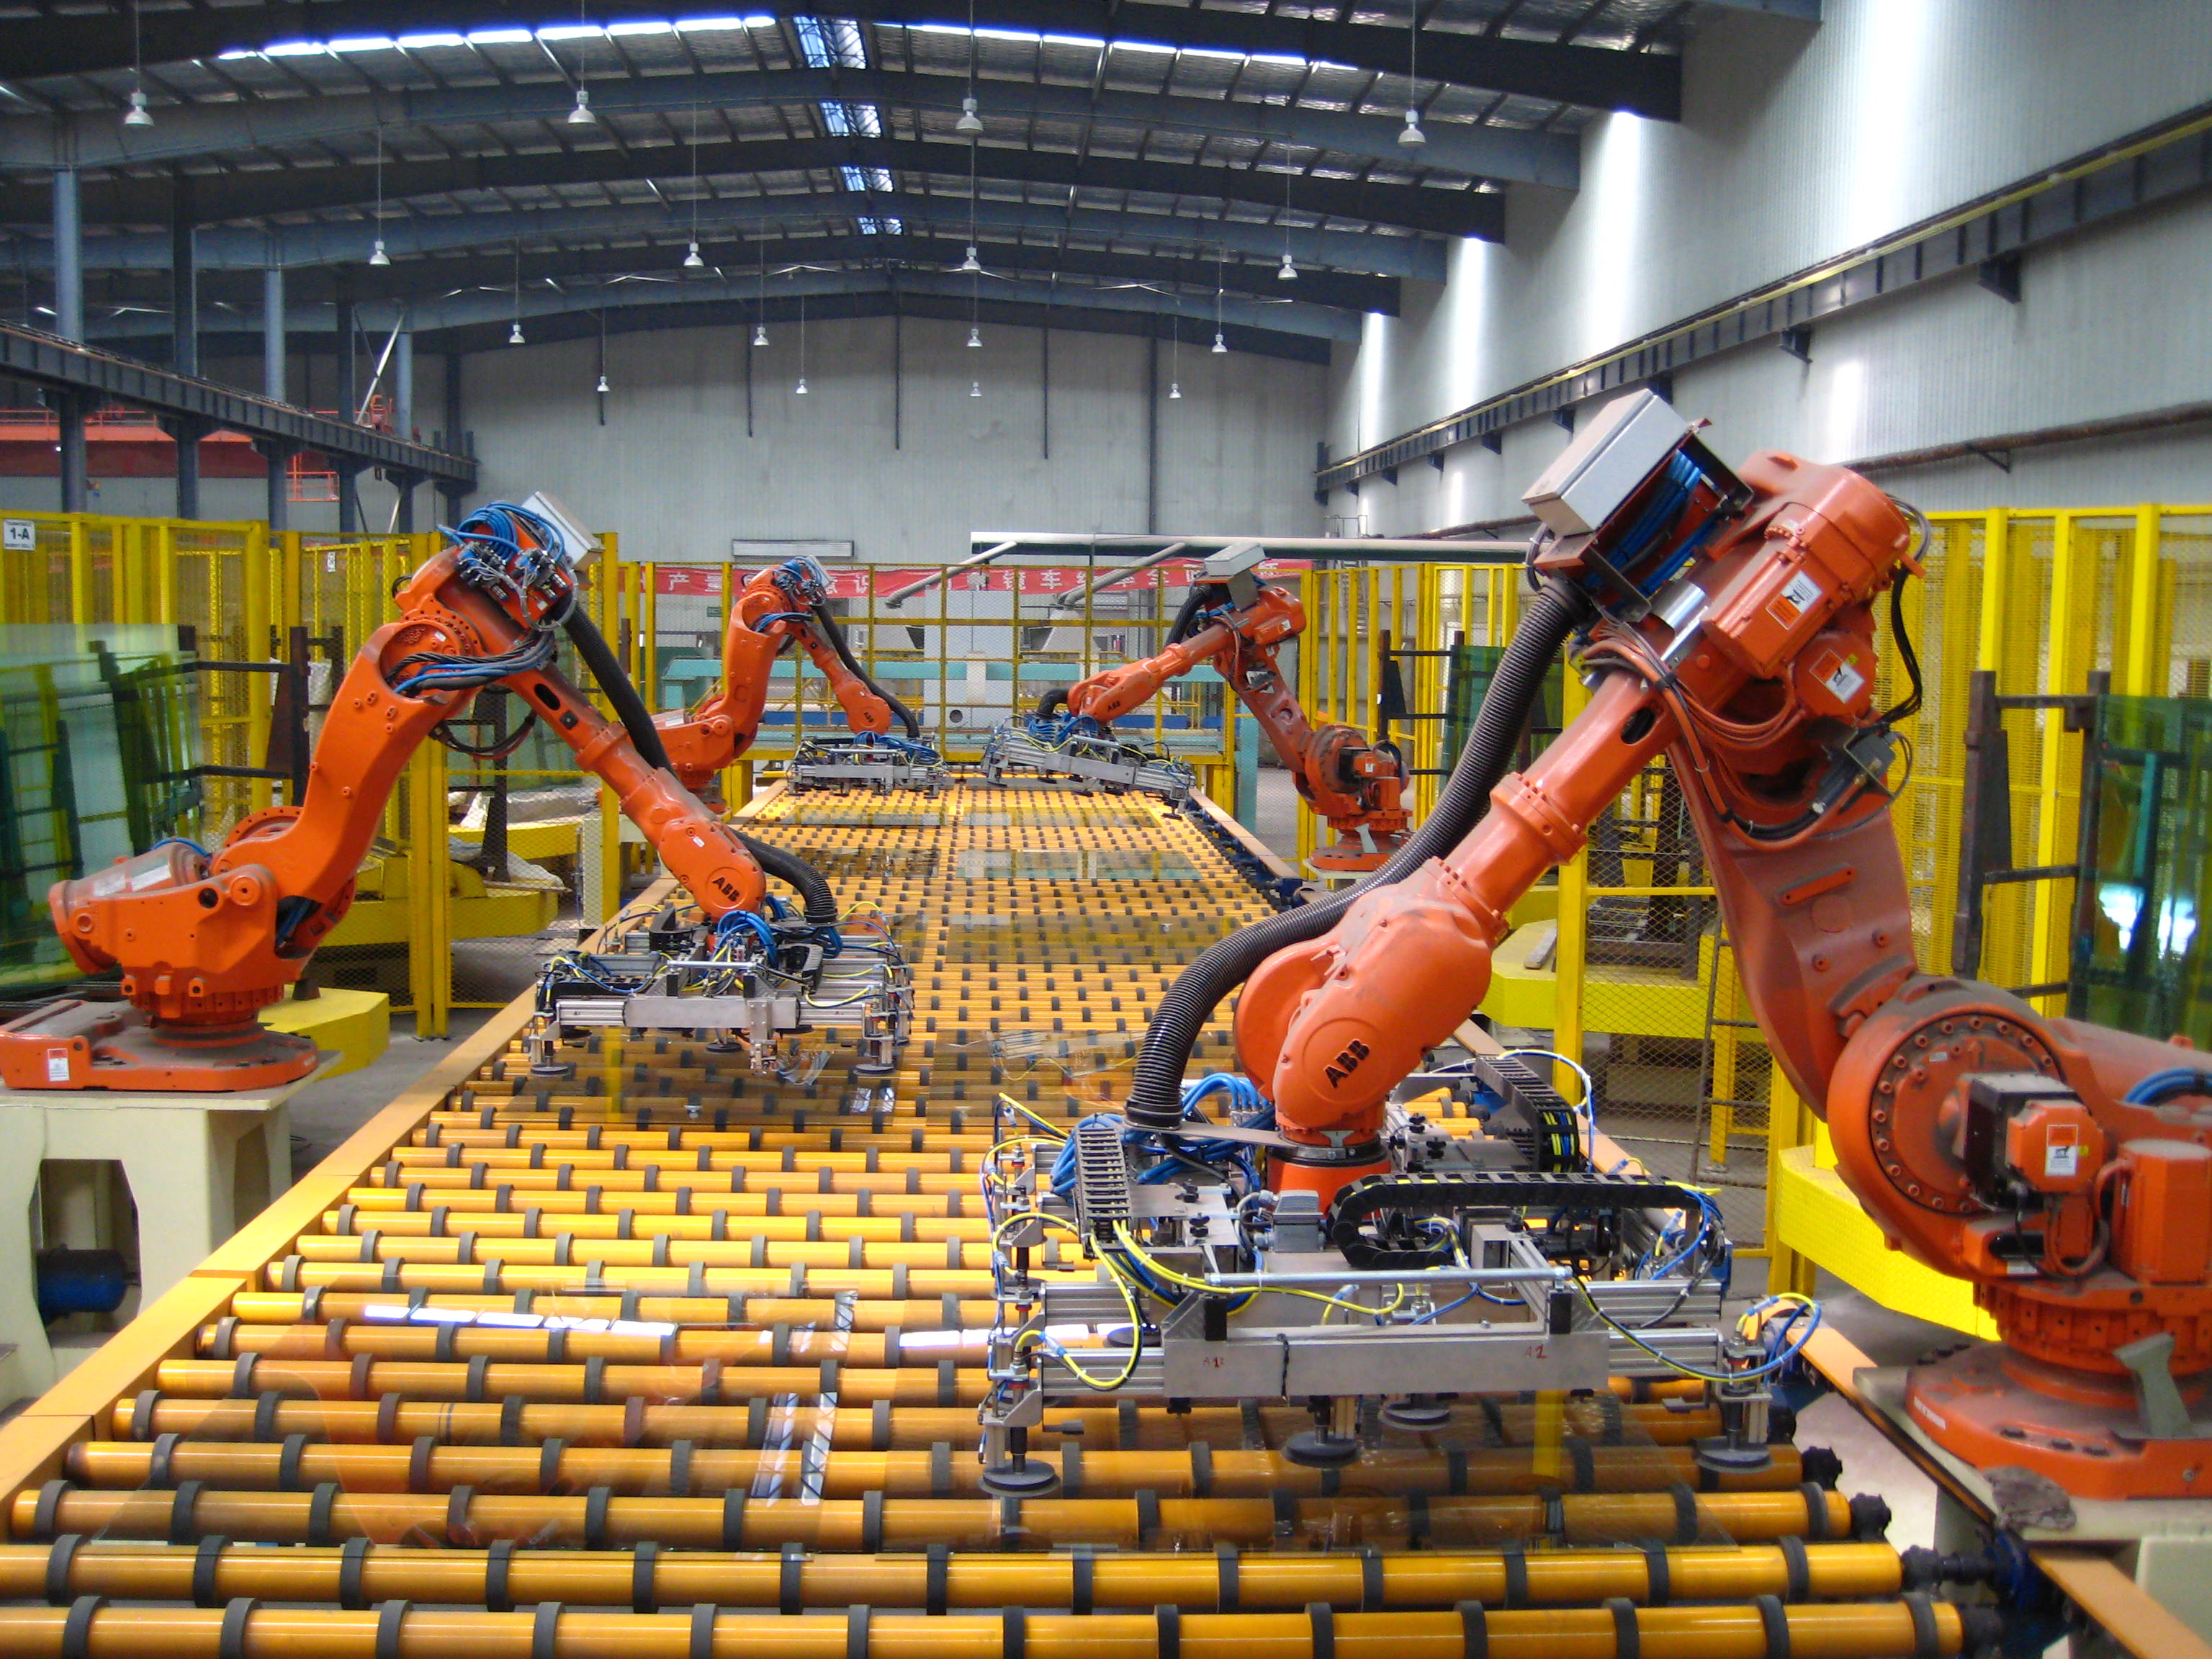
\includegraphics[width=8cm]{figs/industrial_robot.jpg}
    \end{center}
    \caption{Robots en lineas de ensamblaje}
    \label{fig:robIndustrialChain}
  \end{figure}\   

  \item \textit{Soldadura.} Es utilizada en soldadura de estructuras mecánicas debido a su alta precisión y capacidad de realizar 
                            la misma soldadura perfecta una y otra vez. Además, también son usados para soldar placas de circuitos.
  \begin{figure} [h!]
    \begin{center}
      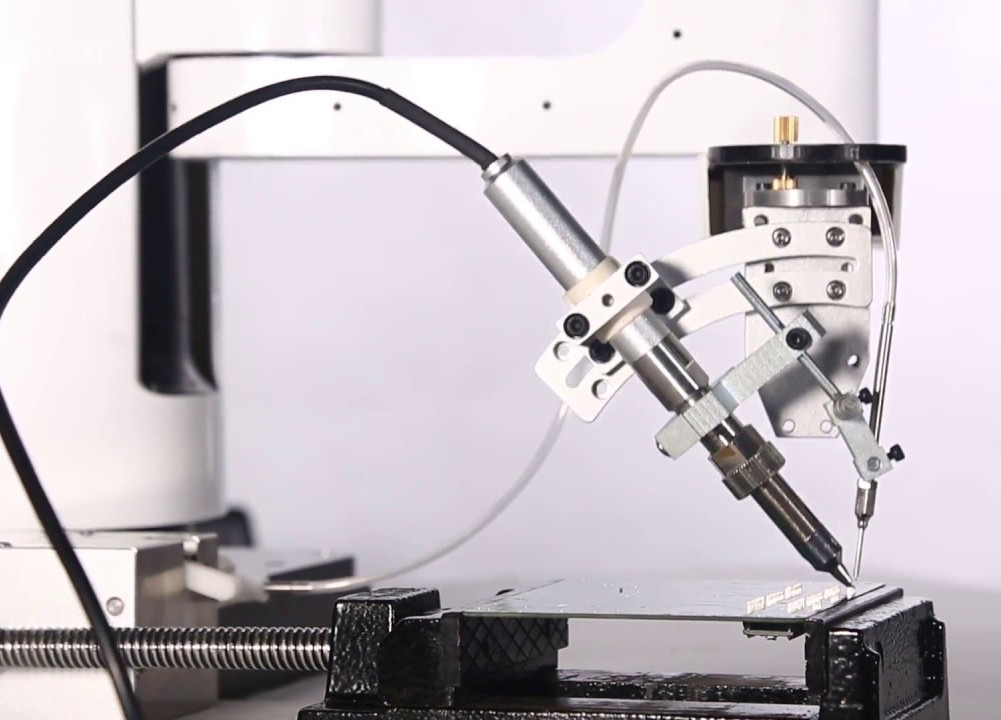
\includegraphics[width=8cm]{figs/solder_robot.jpg}
    \end{center}
    \caption{Robot Dobot M1 realizando una soldadura con estaño}
    \label{fig:robSoldering}
  \end{figure}\ 

  \item \textit{Investigación y desarrollo en laboratorios.} Los brazos robóticos realizan tareas de laboratorio repetitivas y precisas, 
                              lo que puede acelerar el proceso de investigación y desarrollo de nuevos productos médicos. Uno de los usos más 
                              frecuentes es preparar y procesar muestras en investigaciones científicas. En concreto, pueden desempeñar tareas
                              como la extracción de ADN, la separación de componentes, la adición de reactivos y el análisis de muestras 
                              químicas, entre otros. Esto ayuda a reducir los errores humanos y garantizar la integridad y reproducibilidad 
                              de los experimentos llevados a cabo.
  
  \begin{figure} [h!]
    \begin{center}
      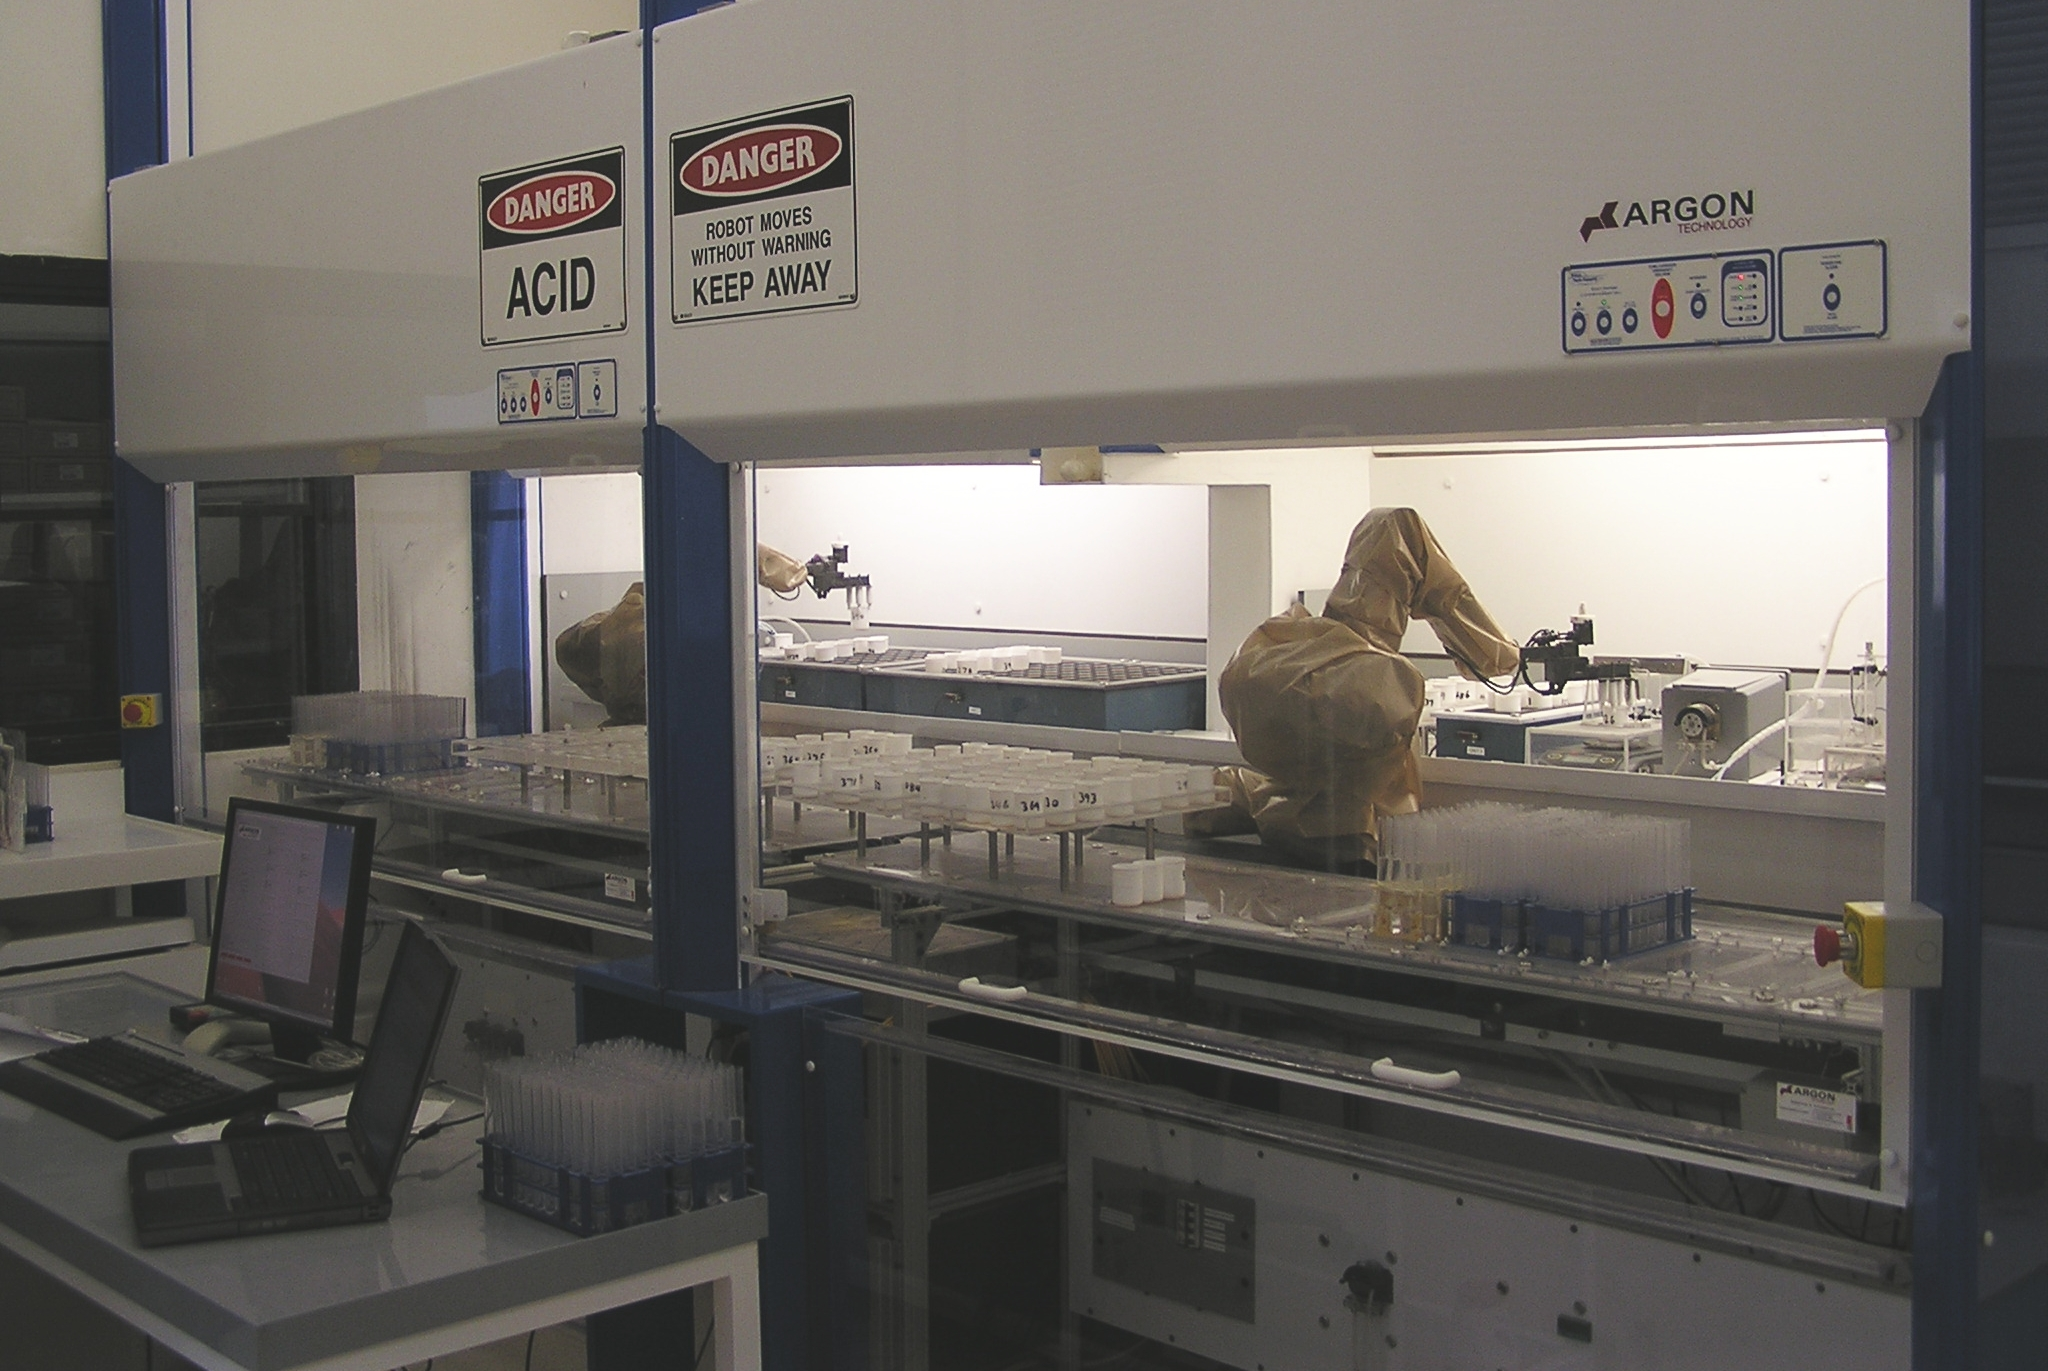
\includegraphics[width=8cm]{figs/lab_robot.jpg}
    \end{center}
    \caption{Robots en el ámbito científico}
    \label{fig:robLaboratory}
  \end{figure}\ 

 \end{itemize}\



\section{Robótica en educación}
\label{sec:segundaseccion}
La robótica en la educación es una disciplina que ha cobrado una gran relevancia en los últimos años debido a la creciente necesidad 
de formar a las nuevas generaciones en competencias tecnológicas. 
\\En las escuelas de secundaria, se ha convertido en una herramienta pedagógica eficaz para desarrollar habilidades y conocimientos en áreas como la programación, 
la matemática, la electrónica y la resolución de problemas. Esto es conocido como \textit{STEM} (Science, Technology, Engineering and Mathematics). Los 
estudiantes aprenden a diseñar, construir y programar robots simples para llevar a cabo una tarea específica, lo que les ayuda a comprender  
los conceptos de ciencia y tecnología de una manera más práctica e interactiva.\\
\begin{figure} [h!]
  \begin{center}
    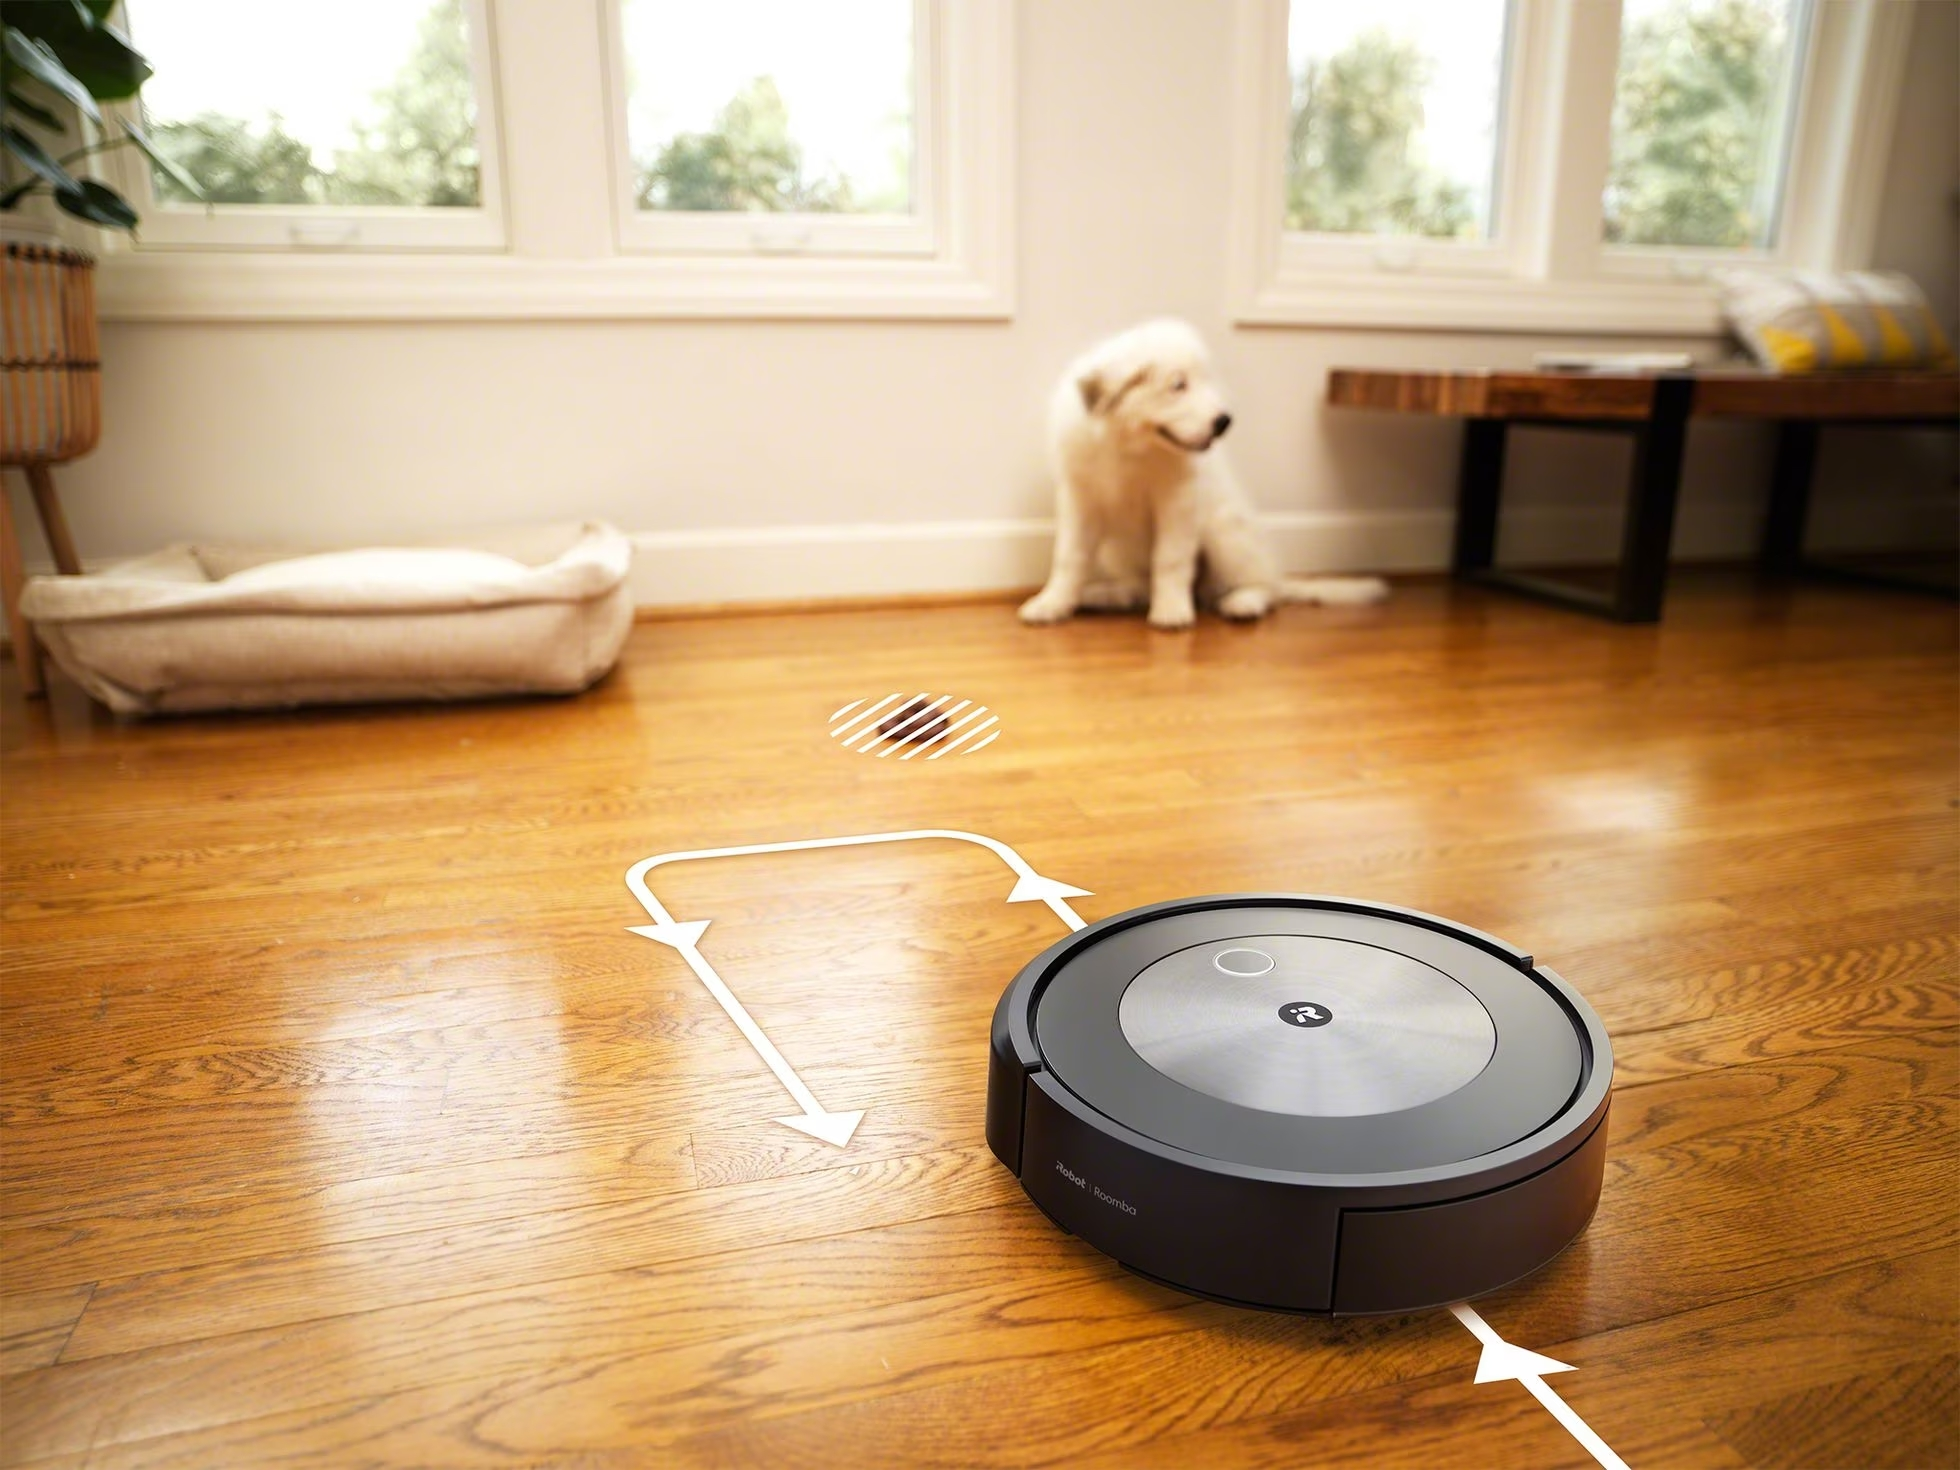
\includegraphics[width=8cm]{figs/roomba}
  \end{center}
  \caption{Robots educativos en la escuela secundaria.}
  \label{fig:robSecundaria}
\end{figure}\
\\En el nivel universitario, la robótica se ha convertido en una disciplina esencial para formar a los futuros ingenieros. Los estudiantes aprenden 
a diseñar y construir robots más avanzados, y refuerzan sus habilidades de programación y control de sistemas complejos. Además se hacen uso de más tipos 
de robot, como pueden ser, industriales o plataformas robóticas móviles reales. Al ser sistemas usados en el mundo profesional, los estudiantes pueden 
aprender con el robot que usará en un futuro. Aunque es verdad que las universidades disponen de algunas unidades, no siempre son accesibles para el 
estudiante por diversas razones.
\newpage

\\En resumen, la robótica en la educación es una herramienta poderosa para fomentar el aprendizaje y la innovación en las nuevas 
generaciones. Desde la escuela hasta la universidad, la robótica se ha convertido en una disciplina clave para formar a los futuros 
líderes tecnológicos del mundo.

No olvides incluir imágenes y referenciarlas, como la Figura \ref{fig:robUniversidades}.

\section{Robótica de bajo coste}
\label{sec:segundaseccion}
La robótica de bajo coste es un área de la robótica enfocada en el diseño y desarrollo de robots 
accesibles y asequibles. El objetivo principal de la robótica de bajo coste es conseguir desarrollar tecnología robótica
barata, reduciendo la complejidad de los sistemas empleados y haciendo uso de materiales más económicos.

La disponibilidad de herramientas de fabricación de bajo costo, como la impresión 3D y el corte láser, 
han hecho posible que los usuarios puedan crear piezas y componentes robóticos personalizados a un 
precio más bajo que el de la fabricación tradicional.

La Ley de Moore es una ley teórica que establece que la capacidad de procesamiento de los microchips se duplica 
cada dos años. Esta observación, pese haberse dado hace casi 60 años, sigue siendo válida a día de hoy. Entre 
otras cosas, es lo que ha permitido el desarrollo de componentes electrónicos cada vez más pequeños, eficientes 
y potentes. La robótica de bajo coste es un claro ejemplo de cómo el crecimiento de la capacidad de computación y 
la disminución de los costes de producción ha llevado al abaratamiento de la robótica y de la electrónica en general.

Gracias a esto, la robótica de bajo coste, se basa en la filosofía `Hazlo tú mismo` o \textit{Do It by Yourself (DIY)} , que se enfoca en la creación de proyectos personalizados y 
asequibles utilizando tecnología de bajo costo y materiales comunes.

En resumen, la robótica de bajo costo es una consecuencia directa del crecimiento de la capacidad de computación, 
el abaratamiento de los precios de los componentes electrónicos y del enfoque \textit{DIY}. Estoque ha permitido la creación 
de robots avanzados y accesibles para el público general.
El desarollo de esta tecnología, permite que más personas puedan experimentar en este área de la ingeniería y desarrollar 
sus propias soluciones robóticas. 
 
\ref{sec:miseccion}

Para hablar de números, mételos en el entorno \textit{math} de \LaTeX, por ejemplo, $1.5Kg$. También puedes usar el símbolo del Euro como aquí: 1.500\euro.

\subsection{Listas}

Cuando describas una colección, usa \texttt{itemize} para ítems o \texttt{enumerate} para enumerados. Por ejemplo:

\begin{itemize}
 \item \textit{Entorno de simulación.} Hemos usado dos entornos de simulación: uno en 3D y otro en 2D.
 \item \textit{Entornos reales.} Dentro del campus, hemos realizado experimentos en Biblioteca y en el edificio de Gestión.
\end{itemize}\


\paragraph{Referencias bibliográficas}
\label{sec:referencias}

Cita, sobre todo en este capítulo, referencias bibliográficas que respalden tu argumento. Para citarlas basta con poner la instrucción \verb|\cite| con el identificador de la cita. Por ejemplo: libros como \cite{vega12e}, artículos como \cite{vega19b}, URLs como \cite{vega19a}, tesis como \cite{vega18b}, congresos como \cite{vega18a}, u otros trabajos fin de grado como \cite{vega08b}.

Las referencias, con todo su contenido, están recogidas en el fichero \texttt{bibliografia.bib}. El contenido de estas referencias está en formato \texttt{BibTex}. Este formato se puede obtener en muchas ocasiones directamente, desde plataformas como \texttt{Google Scholar} u otros repositorios de recursos científicos.

Existen numerosos estilos para reflejar una referencia bibliográfica. El estilo establecido por defecto en este documento es APA, que es uno de los estilos más comunes, pero lo puedes modificar en el archivo \texttt{memoria.tex}; concretamente, cambiando el campo \verb|apalike| a otro en la instrucción \verb|\bibliographystyle{apalike}|. 

\

\

\

Y, para terminar este capítulo, resume brevemente qué vas a contar en los siguientes.


\chapter{Estado del arte}
\label{cap:capitulo2}
\noindent En este capítulo se describen algunos de los trabajos más relevantes publicados sobre robots industriales en educación.

En \cite{KRIMPENIS2020103} se presenta una solución industrial barata para crear un robot capaz de hacer operaciones de mecanizado (fabricación 
de piezas mediante operaciones de corte). Este robot se llama HydraX y esta dotado de 6 grados de libertad. Tiene un alcance máximo de casi un metro, un 
peso que ronda los 13 Kg y está fabricado mediante impresión 3D. 
Además, tiempo después, se publicó la segunda parte de este artículo \cite{PAPAPASCHOS2020109}, en el cual se aborda el diseño software y de control 
que se ha desarrollado para controlar dicho brazo. \\
    \begin{figure} [h!]
        \begin{center}
          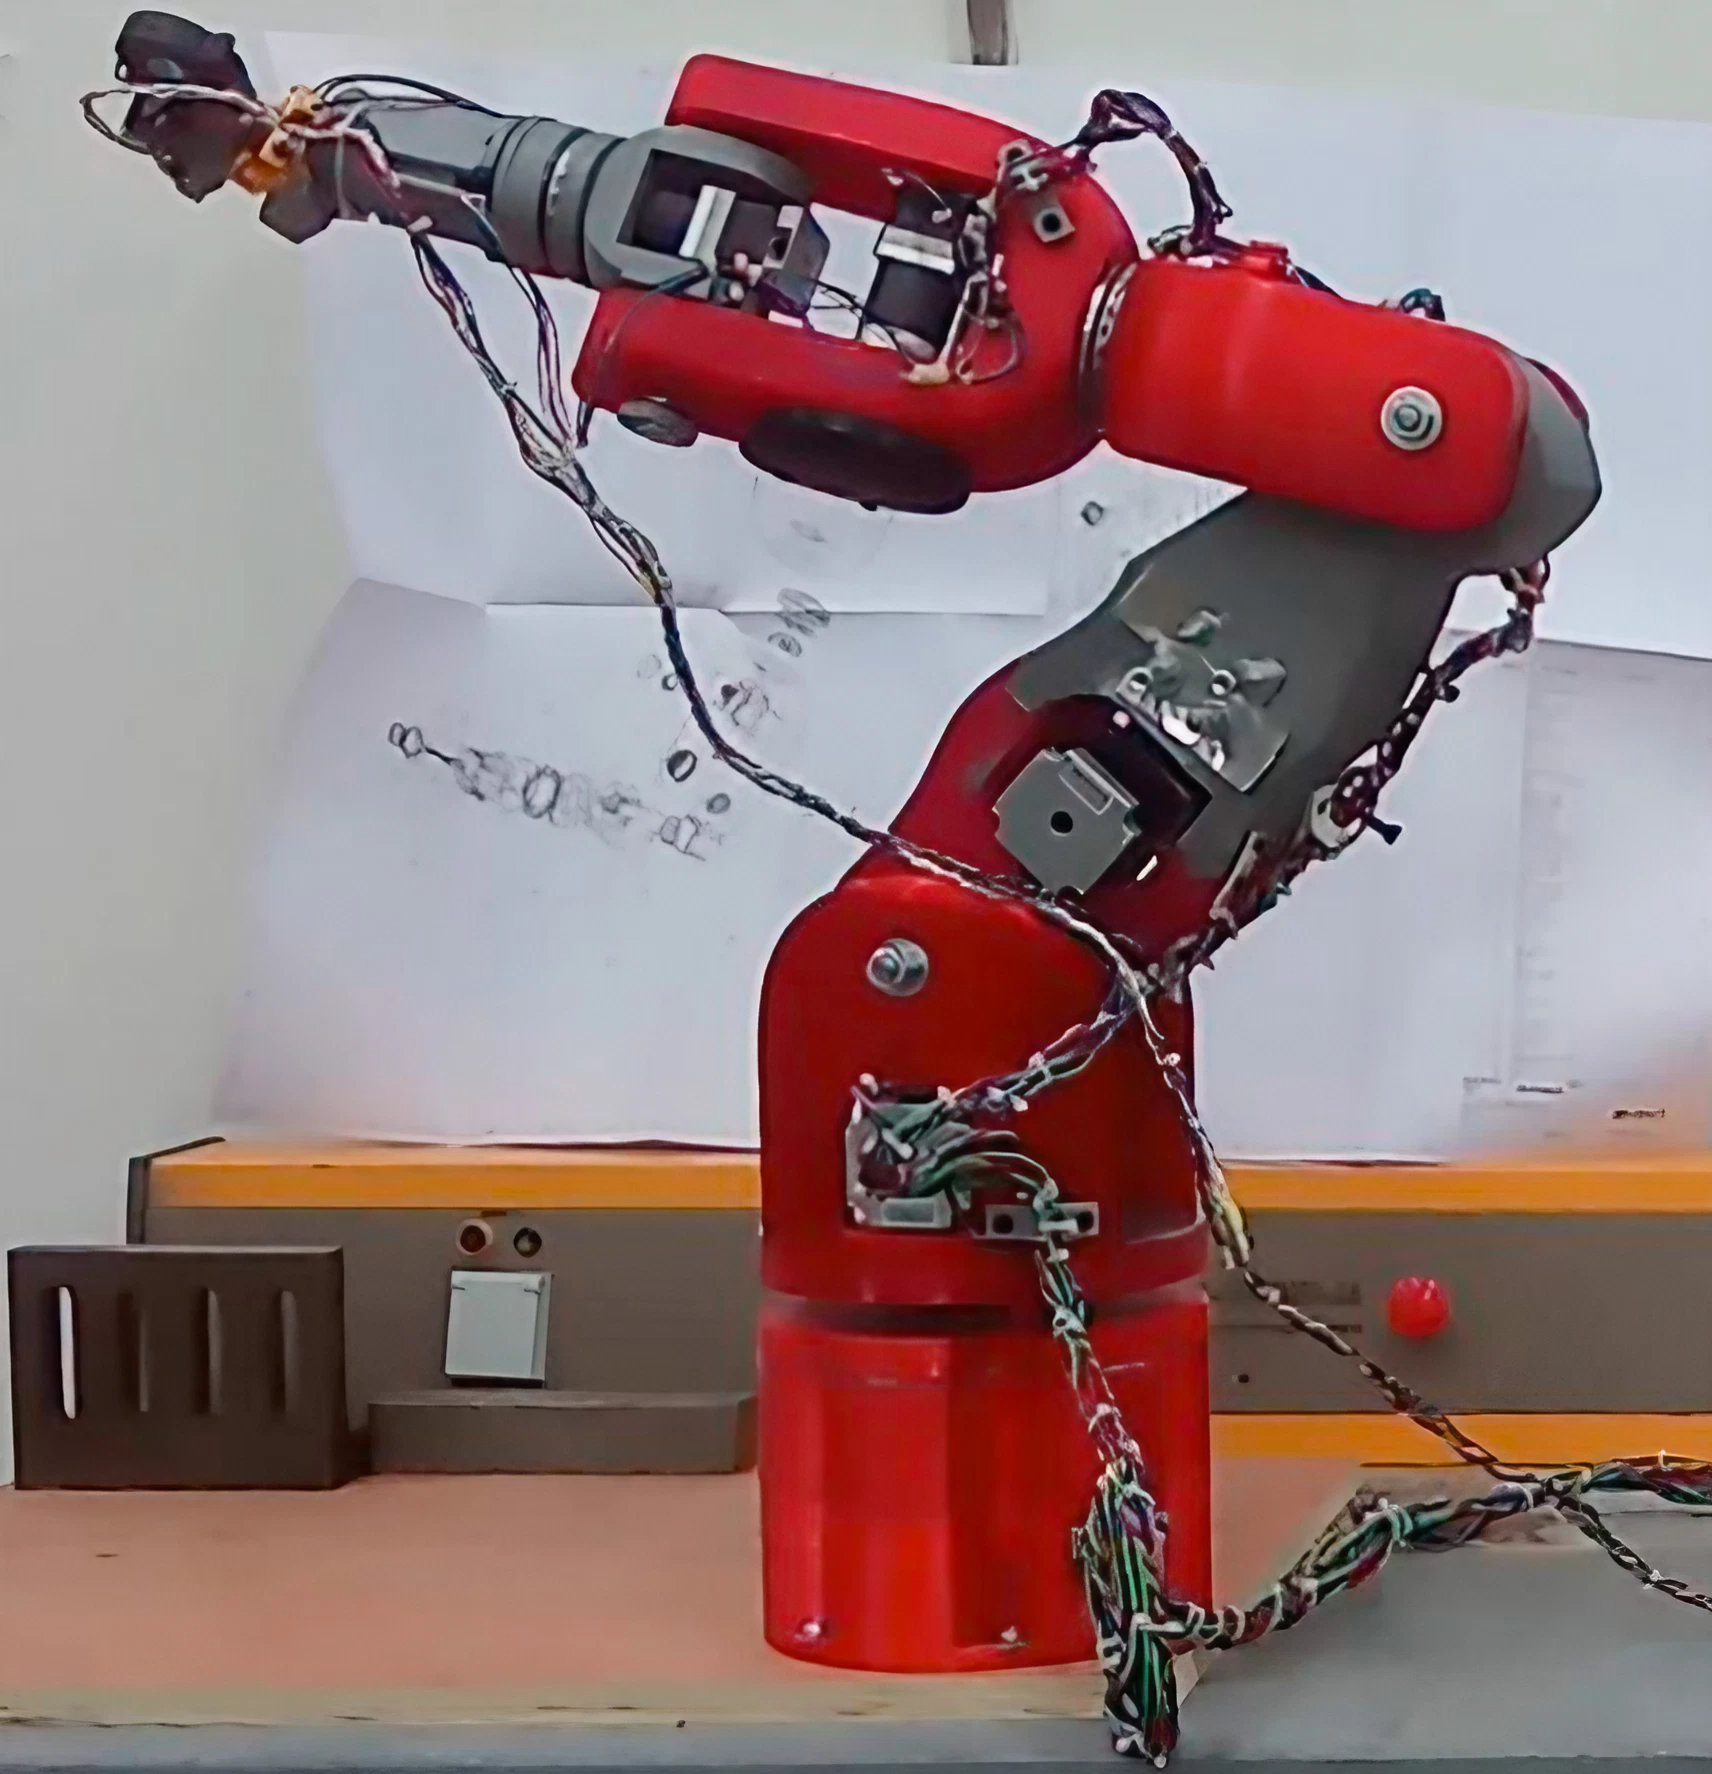
\includegraphics[width=6cm]{figs/Hydra.png}
        \end{center}
        \caption{Robot HydraX}
        \label{fig:hydra}
    \end{figure}\ 
    \newpage
    Los puntos fuertes del proyecto son los siguientes:
    \begin{itemize}
        \item Tiene una repetitividad de ±0.04 mm.
        \item Tiene un espacio de trabajo muy amplio.
        \item Tener más de 3 grados de libertad le permiten alcanzar gran cantidad de puntos con distintas orientaciones.
        \item Según el artículo, tiene una capacidad de carga máxima de 12 kilogramos. A pesar de esto, se comenta que en la práctica el peso en el 
        extremo del robot debe ser menor a 5 Kg, por lo que su carga útil rondará los 3 Kg para un funcionamiento aceptable. Esto lo sitúa a la par 
        del robot comercial ABB IRB 120\footnote{\url{https://new.abb.com/products/es/3HAC031431-001/irb-120}}  
    \end{itemize}\
    
    Y estos son los puntos débiles que cabe mencionar:
    \begin{itemize}
        \item Carece de integración en \ac{ROS}, plataforma de desarrollo de la que se habla en la Sección \ref{subsec:ros2}.
        \item Su coste en materiales supera los 1000 \euro \xspace , por lo que no es lo suficientemente asequible para su uso académico.
        \item Según este artículo, se necesitan 200 horas para poder imprimir y montar el brazo, lo que implica que es costoso en tiempo 
        crear varias unidades, además de que requiere de cierta habilidad para construirlo correctamente.
        \item En este artículo no se proporcionan los ficheros necesarios para poder crearlo. Además, se menciona que las piezas han sido 
        diseñadas mediante el software privativo SolidWorks\textsuperscript{\tiny\textregistered}, por lo que lo hace más difícil y costoso de editar.
    \end{itemize}\
    \newpage
    Existen soluciones más sencillas y reproducibles, como por ejemplo, la presentada en \cite{adediran2023uiarm}. En este trabajo se describe 
    un brazo robótico 
    cuyo propósito es separar botellas de plástico en un proceso de reciclaje. Más allá de la aplicación que se le pretende dar, 
    lo mas importante es que se hace uso de  
    un manipulador de tamaño reducido, impreso en 3D y con 4 \ac{DOF}.
    \begin{figure} [ht!]
        \begin{center}
          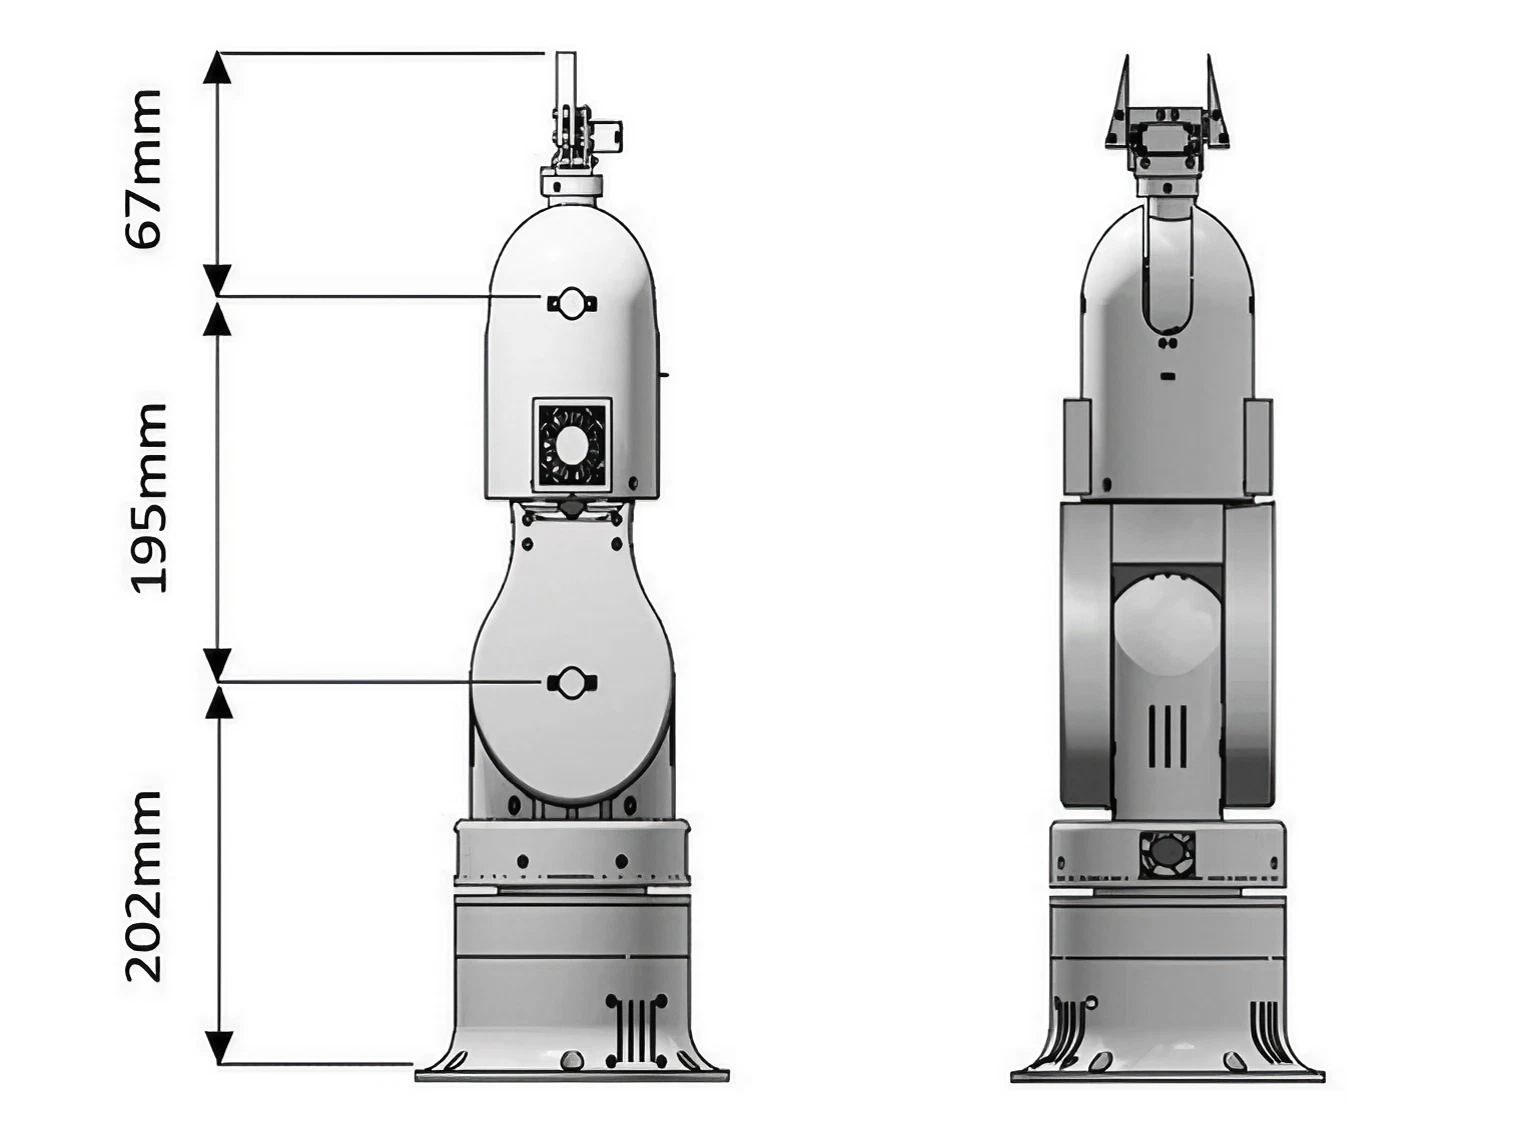
\includegraphics[width=8cm]{figs/uiarm.png}
        \end{center}
        \caption{Robot UIArm}
        \label{fig:uiarm}
    \end{figure}\ 
    
    A partir de la información proporcionada en este artículo, se han extraído los siguientes puntos fuertes:
    \begin{itemize}
        \item El diseño de las piezas se ha realizado mediante el uso de la herramienta de diseño \nameref{subsec:freecad}, esto supone una ventaja respecto 
        a \cite{KRIMPENIS2020103}, que utilizaba una herramienta privativa.
        \item Utiliza motores de pequeño tamaño con una reductora integrada, lo que aumenta su torque y abarata en gran medida los costes 
        del robot. Debido a esto, el consumo de energía es menor pudiendo hacer uso de una electrónica compacta y menos costosa.
        \item Al estar compuesto por menos piezas y tener pocos grados de libertad, se requiere menos tiempo para imprimir y construir este robot.
    \end{itemize}\
    Y estos son puntos negativos que cabría destacar:
    \begin{itemize}
        \item El espacio de trabajo (puntos del espacio alcanzables por el extremo del brazo) del robot es demasiado reducido. Esto es debido 
        a la disposición de los grados de libertad. Utiliza dos de ellos para cambiar la orientación del extremo del robot, dejando solo dos para el 
        posicionamiento, por lo que es imposible en la práctica abarcar todo el espacio 3D al alcance del brazo.
        \item Utiliza engranajes impresos en 3D para rotar la segunda articulación comenzando desde la base. Debido a esto, pierde exactitud en función 
        de la posición del brazo debido a la holgura de este tipo de transmisión.
        \item Carece de integración con \ac{ROS} y el autor no proporciona otro tipo de software que permita desarrollar programas para este robot perjudicando la 
        continuidad del proyecto.
    \end{itemize}\

    Otro desarrollo \textit{low-cost} que ha adquirido gran popularidad
    gracias a la plataforma KickStarter \footnote{\url{https://www.kickstarter.com/projects/niryo/niryo-one-an-open-source-6-axis-robotic-arm-just-f/description}} 
    es el robot Niryo One, que es un brazo robot impreso en 3D con 6 grados de libertad, en la cual fue 
    capaz de recaudar 80.000\euro \xspace de los 20.000 \euro \xspace necesarios. 


    Este proyecto busca dar una alternativa de bajo coste al robot convencional usado por \textit{makers}, estudiantes y 
    pequeñas compañías. Para lograrlo, apuesta por el uso de componentes comunes y la filosofía \textit{Open Source}, la cual se basa en la 
    idea de compartir, colaborar y democratizar el acceso al conocimiento y al software. Por ello, su código fuente y planos están disponibles 
    de forma gratuita para que cualquier persona interesada pueda acceder a ellos.

    Aunque este modelo no es el más nuevo de la marca Niryo, sí es el que más comunidad tiene y más extendido está.
    Este robot y los modelos posteriores, pueden ser adquiridos a través de su página oficial \footnote{\url{https://niryo.com/products-cobots/niryo-one/}}.
    \\
    \begin{figure} [ht!]
        \begin{center}
          
\includegraphics[width=11cm]{figs/niryo.png}
        \end{center}
        \caption{Robot Niryo One}
        \label{fig:niryo}
    \end{figure}\ 
    \newpage
    Este proyecto destaca positivamente por:
    \begin{itemize}
    \item El proyecto completo es de código abierto y se puede encontrar toda la electrónica necesaria y documentos para imprimirlo en 
    su repositorio de github \footnote{\url{https://github.com/NiryoRobotics/niryo_one}}.
    \item Tiene integración con ROS 1 y MoveIt.
    \item Cuenta con 6-DOF, lo que permite alcanzar gran cantidad de puntos con distintas orientaciones.
    \item Cuenta con una repetitividad de 0.5mm y puede levantar hasta 300g.
    \item Permite adaptar una gran variedad de herramientas diferentes.
    \item Es capaz de detectar colisiones gracias a sus motores codificados mediante sensores magnéticos.
    \end{itemize}
    En cambio, tiene los siguientes inconvenientes:
    \begin{itemize}
    \item Hace uso de una placa Raspberry Pi en vez de una placa Arduino/Esp32, lo que incrementa el coste del equipo. 
    \item Hablando del precio, el coste de este equipo comprado en su versión en aluminio ronda los 3500\euro. El coste de fabricación 
    de este robot mediante el uso de impresión 3D ronda los 1000\euro \xspace según este artículo \footnote{\url{https://www.zdnet.com/article/this-mini-industrial-robot-is-less-than-1k/}}
    \item Aunque proporcionan los ficheros fuentes del diseño, este ha sido realizado mediante SolidWorks\textsuperscript{\tiny\textregistered} por 
    lo que no puede ser editado sin tener que pagar por el programa.
    \item Pese a tener integración con ROS1, el proyecto no ha sido adaptado de forma oficial para ROS2, por lo que es necesario 
    usar un sistema operativo antiguo (Ubuntu 16.04) del año 2016. O bien utilizar Ros Bridge \footnote{\url{https://github.com/ros2/ros1\_bridge}} 
    para comunicar el ROS 1 de la placa con un  ordenador moderno con ROS 2.
    \end{itemize}
    \newpage
    En el ámbito de los robots caseros, se puede destacar un referente reconocido, MeArm. Se trata de un 
    brazo mecánico de diseño simple y completamente \textit{OpenSource}. De hecho, tal es su repercusión, que miles de personas 
    se han impreso el suyo o creado su propia versión mejorada. Prueba de ello es la cantidad de modificaciones que se han ido subiendo a  
    páginas como Thingiverse\footnote{\url{https://www.thingiverse.com/search?q=mearm&page=1&type=things&sort=relevant}}. Además, existen 
    robots con diferentes nombres basados en el mismo concepto, como puede ser EEZYBotArm, una versión más robusta y atractiva que el original. \\
    Consta de 3 grados de libertad y de una pinza simple. Todos los motores del robots son servomotores de 9 gramos y se basa en el uso de 
    paralelogramos para transferir el movimiento de los motores al extremo del robot, manteniendo el peso de los mismos en la base. 

    \begin{figure} [h!]
        \centering    
        \subfigure[MeArm]{\label{fig:mearm}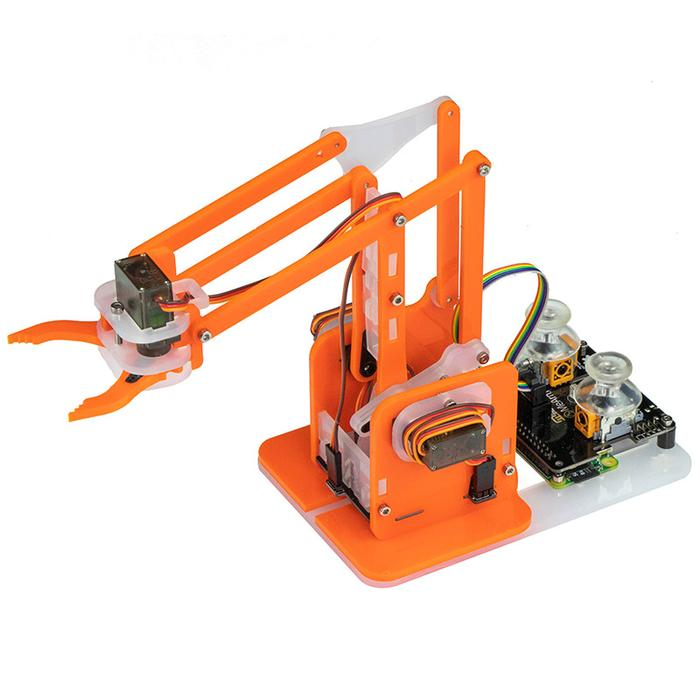
\includegraphics[width=0.3\linewidth ]{figs/mearm.jpg}}
        \hspace{3cm}
        \subfigure[EEZYBotArm MK1]{\label{fig:eezy}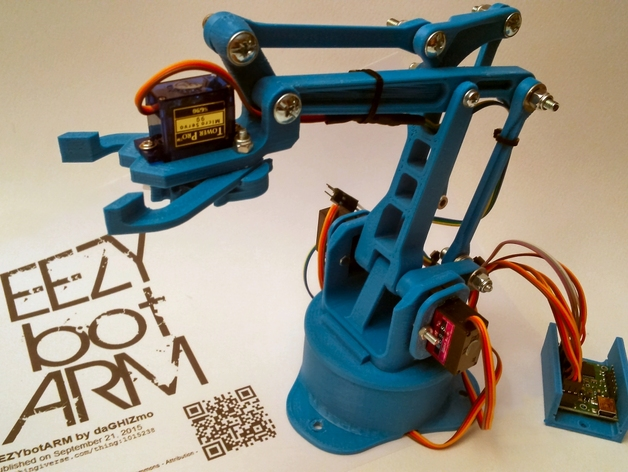
\includegraphics[width=0.3\linewidth]{figs/eezy.jpg}}
        \caption{Robots formados a partir de paralelogramos}
    \end{figure}
    
    Se trata de un proyecto muy extendido, con una comunidad que ha creado muchas variantes de él, por lo que para evaluar los puntos fuertes y 
    débiles del robot, se va a hacer referencia al robot original MeArm V1.
    Los aspectos significativos de este robot son:
    \begin{itemize}
        \item Se trata de un proyecto totalmente accesible y replicable, ya que usa pocos materiales y estos son fáciles de adquirir.
        \item El centro de masa del robot se concentra en la base, reduciendo la inercia del brazo y permitiendo así movimientos más rápidos.
        \item No requiere de apenas tiempo de impresión y el montaje es sencillo gracias a las numerosas guías de 
        montaje\footnote{\url{https://docs.rs-online.com/2bb1/0900766b81593e58.pdf}} que circulan por internet.
        \item Al usar servomotores, se puede establecer el ángulo de cada articulación fácilmente sin necesitar de ningún tipo de sensor externo.
        \item Debido a su forma y materiales utilizados, tiene un peso muy reducido pudiéndose acoplar a robots móviles sin afectar a 
        su rendimiento.
    \end{itemize}
    En cuanto a sus limitaciones, se deben mencionar:
    \begin{itemize}
    \item Se suele prescindir del uso de rodamientos en sus articulaciones. Esto reduce el tiempo de vida del brazo debido a que el propio rozamiento 
    de los ejes acaba desgastando el plástico, creando holguras que afectan directamente en la precisión. Esta holgura obliga a apretar en exceso los tornillos 
    que hacen de ejes de las articulaciones, aumentando el rozamiento y reduciendo fuerza útil de los pequeños motores.
    \item Este robot está limitado en cuanto a fuerza debido al uso de servomotores. Usa los típicos SG90 o similares con un torque de apenas 
    0.16 Newton-metro. El uso de servos más grandes aumenta significativamente el precio del dispositivo. 
    \item Los servomotores padecen de vibraciones al conectarle una carga. Esto hace que el conjunto tiemble en exceso durante los movimientos.
    \end{itemize}

\noindent Una vez se han presentado los proyectos más relevantes en este campo, se procederán a definir una serie 
de requisitos y objetivos concretos para dar solución al problema que se plantea en este trabajo.


\chapter{Objetivos}
\label{cap:capitulo3}

\begin{flushright}
\begin{minipage}[]{10cm}
\emph{Un objetivo sin un plan es solo un deseo}\\
\end{minipage}\\

Antoine de Saint-Exupéry\\
\end{flushright}

\vspace{1cm}

Tras haber enmarcado el contexto en el cual se encuentra este trabajo de fin de grado, se procede a realizar
una descripción del problema, requisitos, metodología y plan de trabajo usado.
\section{Descripción del problema}
\label{sec:descripcion}
Este trabajo de fin de grado nace de la necesidad de abordar el problema existente en nuestra universidad, donde la escasez de 
robots disponibles y la dificultad para acceder a ellos han limitado nuestra experiencia práctica en robótica. 
Estos dispositivos son costosos, lo que limita su disponibilidad, y su fragilidad impide que los estudiantes 
interactúen plenamente con ellos por temor a dañarlos. Además, la cantidad limitada de robots en relación con el número de carreras que 
quieren utilizarlos, crea una gran competencia por su uso. Sumado a ello, los profesores tienen que hacer frente a la burocracia asociada al 
uso de los mismos. 
La solución propuesta busca superar estas limitaciones al proporcionar a la enseñanza un robot casero impreso en 3D, que será
económico, accesible y útil en el aprendizaje práctico de los estudiantes. 
Por lo tanto, el objetivo principal de este trabajo de fin de grado es desarrollar un brazo robótico que pueda ser empleado en la 
asignatura de Robótica Industrial de esta universidad. Asimismo, se busca que el sistema creado sea asequible y fácilmente replicable haciendo uso de las impresoras 3D de la universidad.\\
Con el fin de alcanzar esta meta, se ha dividido el proyecto en los siguientes subobjetivos:

\begin{enumerate}
    \item Realizar una investigación acerca de los robots que actualmente están disponibles y que cumplan con 
          las características y objetivos deseados. Estos robots deberán tener un tamaño y costo similar, y 
          preferiblemente haber sido impresos en 3D. Se dará mayor relevancia a aquellos que utilicen un software y hardware 
          libres.
    \item Explorar diversas opciones de diseño para determinar la forma ideal del robot. Se analizará cuidadosamente 
          qué tipo de robot se ajusta mejor al uso que se le pretende dar, así como los grados de libertad necesarios. 
            
    \item Realizar una investigación exhaustiva sobre los componentes de hardware disponibles en el mercado, con el fin de seleccionar 
          aquellos que mejor se adapten a las necesidades y objetivos de construir un robot eficiente y funcional. Se llevará 
          a cabo un análisis detallado de los precios y características de cada componente, para seleccionar aquellos 
          que ofrezcan la mejor relación calidad-precio. Una vez evaluados todos los aspectos, se elegirá un conjunto 
          final de componentes para construir el robot de manera efectiva. 
    
    \item Realizar el \ac{CAD} del brazo. Se pretende hacer uso de FreeCad\footnote{\url{https://www.freecad.org/index.php?lang=es_ES}}, entre otras herramientas, para
          diseñar en 3D cada pieza que constituirá el robot. Puesto a que debe ser imprimible en una impresora \acs{FDM} convencional,
          debe estar pensado para no necesitar soportes y utilizar el mínimo material posible.
    \item Emplear una impresora 3D convencional para materializar los diseños realizados anteriormente.
    \item Programar el software necesario para poder controlar el robot desde el ordenador.
    \item Realizar la integración del robot realizado en el ecosistema \ac{ROS}. 

  
\end{enumerate}\


\section{Requisitos}
\label{sec:requisitos}
Con el fin de solucionar el problema descrito, se han establecido los siguientes requisitos:
\begin{enumerate}
      \item Se espera un brazo robot de tipo industrial de bajo coste cuya fabricación completa esté por debajo de 200\euro.
      \item La mayoría de las partes que componen el robot, deben ser imprimibles en cualquier impresora 3D convencional.
      \item A fin de poder garantizar la portabilidad del robot, este debe de tener un consumo inferior a 25 vatios.
      \item En cuanto a sus dimensiones, se busca un tamaño idóneo para su uso sobre un escritorio. Esto implica que no necesariamente 
      tiene que estar unido al suelo, permitiendo su fácil traslado.
      \item Es necesario que sea simple de montar y esté compuesto del menor número de piezas posibles con el fin de poder crear varias unidades 
      en poco tiempo. 
      \item Se busca continuidad en el proyecto a largo plazo, por lo que debe tener integración con el ecosistema \acs{ROS} 2. 

\end{enumerate}\

\section{Metodología}
\label{sec:metodologia}

Durante el desarrollo del trabajo se ha establecido un protocolo de reuniones semanales con el tutor a 
través de la plataforma Teams, con el objetivo de compartir los avances realizados y recibir retroalimentación 
sobre el trabajo. Además, cada semana se han propuesto las actividades a realizar, asegurando así una adecuada 
planificación y coordinación del proyecto. \\
Para el desarrollo del sistema se ha utilizado un repositorio en la plataforma GitHub\footnote{\url{https://github.com/RoboticsURJC/tfg-vperez}}, en el cual se ha ido
subiendo el código y diseños generados a lo largo del proyecto. Adicionalmente, en este mismo repositorio 
se ha incluido una Wiki\footnote{\url{https://github.com/RoboticsURJC/tfg-vperez/wiki}} con las explicaciones detalladas de todas las actividades llevadas a cabo durante estos 
meses de trabajo. De esta manera, se ha creado un registro completo y accesible de todo el proceso de desarrollo del sistema.

\section{Plan de trabajo}
\label{sec:plantrabajo}
El desarrollo del TFG ha estado dividido en dos etapas. La primera, comenzó en octubre y fue abandonada en enero. 
//TODO

\chapter{Plataforma de desarrollo}
\label{cap:capitulo4}

\begin{flushright}
\begin{minipage}[]{10cm}
\emph{Las herramientas adecuadas en las manos adecuadas pueden cambiar el mundo}\\
\end{minipage}\\
Steve Jobs\\
\end{flushright}

\vspace{1cm}
Tras haber establecido los objetivos que se pretenden alcanzar en este trabajo de fin de grado, se procede a describir
las herramientas \textit{software} y \textit{hardware} utilizadas para lograrlos. 

\section{Software}
\label{sec:software}
Llamamos \textit{software} al conjunto de programas, instrucciones y datos que dotan de lógica al sistema.
\subsection{Python}
\label{subsec:pyhton}
Python es un lenguaje de programación, es decir, una serie de reglas gramaticales bien definidas que le proporciona a una persona, en este 
caso el programador, la capacidad de programar una serie de instrucciones o secuencias de órdenes con el fin de crear un comportamiento 
lógico determinado. 

Se trata de un lenguaje de alto nivel interpretado. Cuando se dice que un lenguaje es de alto nivel, se hace referencia a su nivel de 
abstracción y facilidad de uso en comparación con los lenguajes de bajo nivel, es decir, aquellos que te permiten mayor control sobre los 
componentes físicos del sistema. Decimos que es un lenguaje interpretado debido a que no es necesario convertir el texto escrito por el humano en 
instrucciones entendibles por un procesador previamente a su ejecución. Esto agiliza el proceso de desarrollo ya que la conversión de código humano a 
código máquina (compilación) suele demorar un tiempo. Por el contrario, la ejecución de un programa en lenguaje compilado es más rápida.  

Una de las características más destacadas de Python es su amplia librería (conjunto de código destinado a un objetivo concreto) estándar, que proporciona 
variedad de módulos y funciones para realizar multitud de tareas. Como cualquier otro lenguaje de programación, cuenta con una gran cantidad de librerías de terceros que 
amplían sus capacidades, como SciPy en la ciencia de datos, Django en el desarrollo web, Numpy para operar con matrices, TensorFlow el aprendizaje automático, entre otros.

\subsection{Grbl}
\label{subsec:grbl}
Grbl\footnote{\url{https://github.com/gnea/grbl}} es un firmware de código abierto usado para controlar máquinas llamadas \acs{CNC}. Este firmware se ejecuta en 
un microcontrolador, que se encuentra dentro de la controladora de la máquina \acs{CNC}, en nuestro caso, la placa base del robot. \\
Básicamente, convierte las instrucciones de código G, que posteriormente hablaremos de él, en señales eléctricas que se envían a los motores de la máquina. Además, 
comprueba los diferentes sensores de la máquina, como pueden ser los finales de carrera, para establecer los límites físicos de cada movimiento. \\
Grbl es flexible por lo que podemos cambiar la configuración para adaptarla a un caso de uso concreto. De hecho, aunque solo soporta movimientos lineales,
en este trabajo se abordará la configuración necesaria para para poder usar las articulaciones rotativas del nuestro robot.
\begin{figure} [h!]
  \begin{center}
    
\includegraphics[width=4cm]{figs/grbl.png}
  \end{center}
  \caption{Logo de Grbl}
  \label{fig:grbllogo}
\end{figure}\ 
\subsection{Código G}
\label{sec:gcode}
\textit{G-code}, también conocido como RS-274, es el nombre del lenguaje de programación más usado en máquinas de \ac{CNC}. 
Proporciona control numérico basado en métricas para equipos controlados por \ac{CAM}, como pueden ser, fresadoras y tornos. 
La programación de este lenguaje precisa de una sintaxis específica en la que se emplean letras y números para representar 
diferentes comandos y parámetros. Por ejemplo, la letra "G" seguida de un número indica un comando de movimiento, mientras 
que la letra "M" seguida de un número se utiliza para comandos misceláneos, como el encendido o apagado del láser/motor de fresado.
Así es como se programan los movimientos necesarios para que la herramienta realice una trayectoria cuadrada en el plano XY:
\begin{verbatim}
  G90       ; Establecer modo de posicionamiento absoluto
  G21       ; Establecer unidad de medida en milímetros
  F200      ; Establecer velocidad de avance a 200 unidades por minuto 
  
  G0 X0 Y0  ; Mover a la posición inicial (esquina inferior izquierda) 
  G1 X20    ; Mover horizontalmente hacia la derecha 20 mm
  G1 Y20    ; Mover verticalmente hacia arriba 20 mm
  G1 X0     ; Mover horizontalmente hacia la izquierda 20 mm
  G1 Y0     ; Mover verticalmente hacia abajo 20 mm
  G0 X0 Y0  ; Volver a la posición inicial (esquina inferior izquierda)
  
  M2        ; Fin del programa
\end{verbatim}

\subsection{FreeCAD}
\label{subsec:freecad}
FreeCAD\footnote{\url{https://www.freecad.org/index.php?lang=es_ES}} es una aplicación de diseño asistido por ordenador de código abierto y gratuita, utilizada para el modelado de piezas en 3D .
Está dirigida al mundo de la ingeniería mecánica y el diseño de productos, pero también es usada en arquitectura y otros campos.
\\FreeCAD utiliza modelado paramétrico. Se trata de un enfoque de diseño que utiliza parámetros y relaciones entre ellos para 
crear modelos 3D modificables, lo que permite realizar un cambio en la geometría modificando el valor de un cierto parámetro.
También ofrece una variedad de bancos de trabajo (\textit{work benches}) especializados, como \textit{Part Design}, \textit{Sketcher} y \textit{Draft} para adaptarse a diferentes 
necesidades de diseño. Además, permite incluir nuevas herramientas y funcionalidades creadas por la comunidad, mediante su administrador 
de complementos.
\\FreeCAD cuenta con una comunidad activa de usuarios que contribuyen al desarrollo y la mejora continua del software. Gracias a esto, 
es sencillo aprender a utilizarlo a partir de las numerosas guías de uso y tutoriales.
\begin{figure} [h!]
  \begin{center}
    
\includegraphics[width=4cm]{figs/freecad.png}
  \end{center}
  \caption{Logo de FreeCAD}
  \label{fig:freecadlogo}
\end{figure}\ 

\subsection{ROS 2}
\label{subsec:ros2}
ROS, por sus siglas en inglés, significa \textit{Robot Operating System}. Se trata de una plataforma de código abierto utilizada 
para desarrollar y controlar sistemas robóticos.
El objetivo principal de ROS es facilitar el desarrollo de sistemas robóticos al proporcionar una infraestructura que permite que
los desarrolladores pueden centrarse en la lógica y el comportamiento específico de los robots, sin tener que preocuparse por la 
infraestructura de comunicación y control. 
Además, proporciona una colección de bibliotecas, herramientas y convenios que permiten a los programadores crear software para robots. 
También proporciona herramientas para la visualización de datos, simulación de robots, depuración y pruebas. Además, 
cuenta con una comunidad activa de usuarios y desarrolladores que contribuyen con paquetes adicionales y comparten su 
conocimiento.

Está diseñado para ser modular, lo que permite la creación de sistemas complejos mediante la reutilización de otros componentes existentes.

Una de las características distintivas de ROS es su arquitectura basada en nodos. Los nodos son procesos independientes 
que se comunican entre sí mediante mensajes. Cada nodo puede realizar tareas específicas, en función de la lógica atribuída por el programador.

En este trabajo se utiliza ROS 2, la versión sucesora de ROS. Esta versión incorpora gran variedad de mejoras respecto a su anterior versión. En esta versión 
los nodos no dependen de un nodo \textit{Master} para comunicarse ya que las comunicaciones están distribuidas mediante el uso de \ac{DDS}. Esto 
incrementa la robusted del sistema y reduce significativamente los tiempos de latencia. \\
La distribución de utilizada en este trabajo es \textit{ROS 2 Humble}. Se trata de la última versión de ROS estable disponible para Ubuntu 22.04 LTS.
\begin{figure} [h!]
  \begin{center}
    
\includegraphics[width=4cm]{figs/ros2logo.jpeg}
  \end{center}
  \caption{Logotipo de ROS 2 Humble}
  \label{fig:ros2logo}
\end{figure}\ 

\subsection{MoveIt!}
\label{subsec:moveit}
MoveIt es una plataforma de desarrollo (\textit{framework}) para manipulación robótica de código abierto que permite desarrollar 
aplicaciones de manipulación complejas utilizando ROS. Además, proporciona una amplia gama de herramientas y bibliotecas que 
facilitan el control y planificación de movimientos de robots. Con MoveIt, puedes crear fácilmente aplicaciones que permitan
a los robots realizar tareas de manipulación avanzadas, como agarrar objetos, ensamblar piezas y mover el brazo en entornos complejos. 
Es altamente flexible gracias a su diseño modular y se puede utilizar con una gran variedad de robots. De hecho, incorpora la herramienta 
\textit{MoveIt Setup Assistant}; se trata de una asistente de configuración con interfaz gráfica que te permite generar los ficheros 
necesarios para utilizar tu propio robot en este ecosistema. 
\begin{figure} [h!]
  \begin{center}
    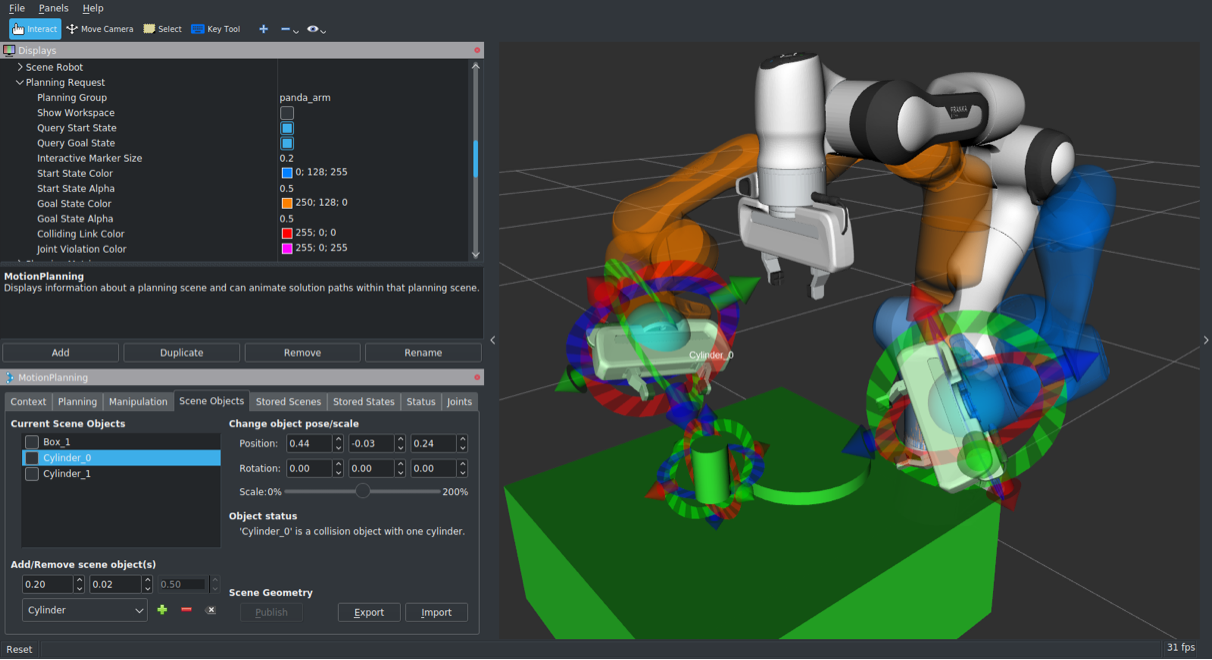
\includegraphics[width=12cm]{figs/moveit_intro.png}
  \end{center}
  \caption{Aspecto del plugin de MoveIt para Rviz2 (Franka Emika Robot)}
  \label{fig:ros2logo}
\end{figure}\ 

\section{Hardware}
\label{sec:hardware}
Cuando hablamos de \textit{hardware}, nos referimos a todos los componentes físicos de utilizados en el dispositivo electrónico, en este caso, un robot. Estos 
componentes son tangibles, es decir, se pueden tocar y ver.

\section{MKS DLC32}
\label{subsec:mksdlc32}
Se trata de una placa destinada al mundo de las máquinas de grabado láser. Ha sido creada por \textit{MakerBase} y es considerada 
\textit{Open Hardware} por lo que toda la información de la placa puede encontrarse en su repositorio de Github\footnote{\url{https://github.com/makerbase-mks/MKS-DLC32}}.
Es fácilmente adquirible por \textit{Aliexpress} por un precio que ronda los 16\euro. Está basada en el microcontrolador de 32 bits: ESP32. 
Se trata de un dispositivo muy asentado en la comunidad \textit{maker} debido a su bajo coste e integración en el 
ecosistema Arduino. De hecho, gracias a su conectividad wifi y bluetooth ha ganado terreno a los microcontroladores Atmega que incorporan los propios Arduinos.\\
Esta placa es ideal para este proyecto debido a que cuenta con la posibilidad de controlar 
hasta 3 motores y es completamente compatible con \nameref{subsec:grbl}. Además dispone de una salida de potencia regulable controlable mediante \nameref{subsec:grbl} que nos 
permite alimentar dispositivos. Estos podrían ser: electroimán (tipo de imán que es activado mediante electricidad), motor \ac{CC} entre otros. Además se puede aprovechar las salidas \ac{PWM} para conectar un grabador láser o un servo. 
El rango de funcionamiento es de 12 a 24 voltios por lo que es adecuado para ser alimentado mediante baterías y con cargadores de ordenador. 
\begin{figure} [h!]
    \begin{center}
      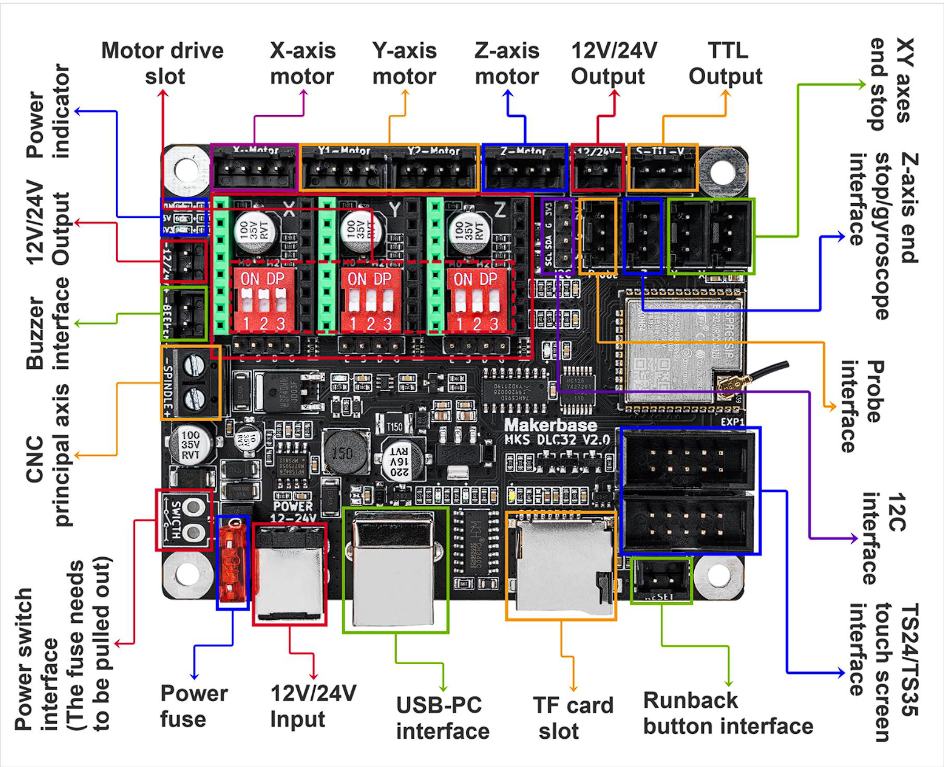
\includegraphics[width=10cm]{figs/MKS.png}
    \end{center}
    \caption{Placa base MakerBase DLC32}
    \label{fig:robSoldering}
  \end{figure}\ 

\section{Motores Nema 17}
\label{subsec:motores}
Un motor paso a paso es un tipo de motor que se mueve en pequeños pasos o incrementos discretos en lugar de girar continuamente. Estos pasos 
son controlados por señales eléctricas que hacen girar al motor una cantidad específica de grados cada vez que se envía una señal. Debido a que se tiene 
control sobre su avance son una excelente opción si se quiere tener un motor que sea capaz de posicionarse en un ángulo concreto con exactitud. A pesar
de su gran precisión, los motores paso a paso convencionales no tienen el conocimiento absoluto de su posición, por lo que todos los movimientos son 
relativos. Esto hace que se requiera de un \textit{homing} (proceso en el cual la máquina CNC lleva las partes móviles a una 
posición conocida) en el arranque de la máquina para conocer su estado antes de operar.
Para este trabajo, se han usado 3 motores Nema 17 de 60 milímetros de largo debido a las necesidades calculadas más adelante. Son motores bipolares de 
2.1 amperios y una resistencia de 1,6 ohmios con un torque máximo de 0.65 newton-metro.
\begin{figure} [h!]
    \begin{center}
      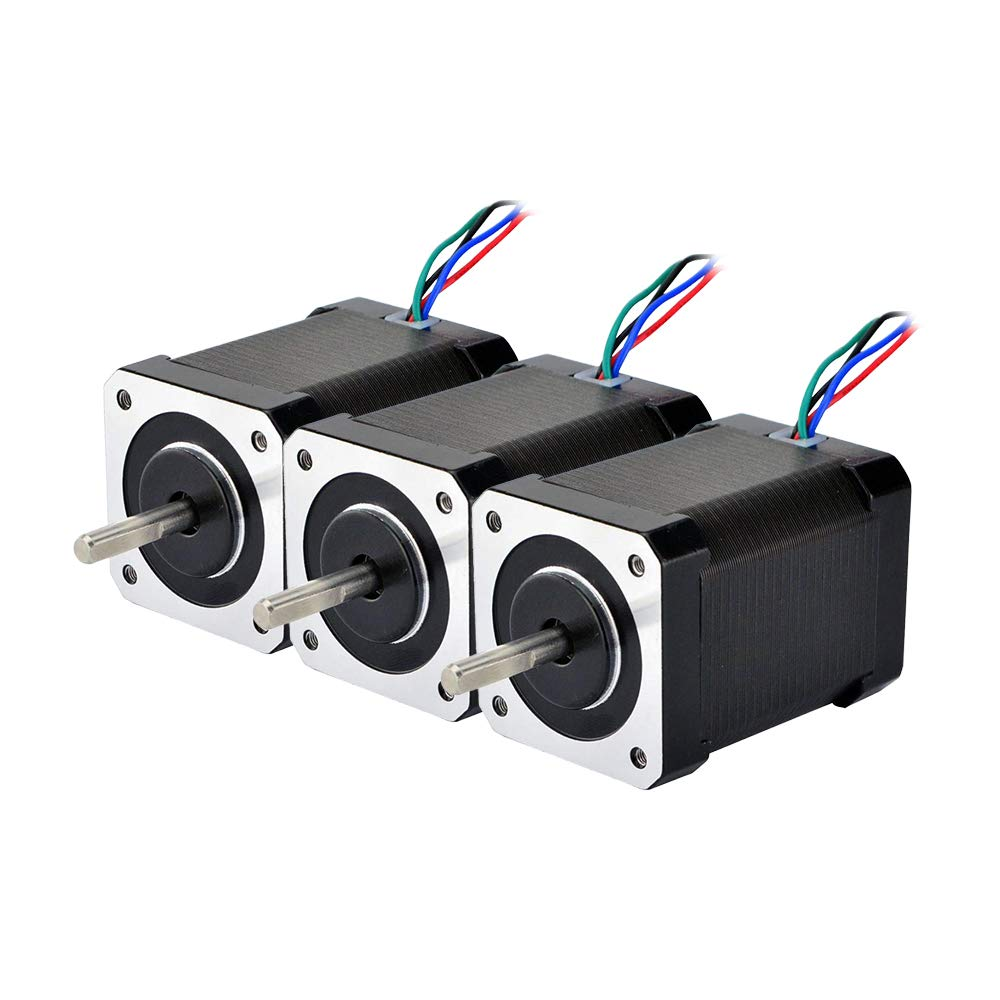
\includegraphics[width=8cm]{figs/nema17.jpg}
    \end{center}
    \caption{Motores Nema 17 de 2.1A}
    \label{fig:robSoldering}
  \end{figure}\ 

\begin{table}[H]
\begin{center}
\begin{tabular}{|c|c|}
\hline
\textbf{Parámetros} & \textbf{Valores} \\
\hline
Nombre del motor & 17HS24-2104S \\
Tipo de motor & Bipolar \\
Ángulo de paso & 1.8º \\
Resistencia de fase & 1.6$\Omega$ \\
Corriente máx. de fase & 2.1A \\
Torque de sujección & 0.65Nm. \\
Dimensiones & 42x42x60mm \\
Peso & 500g \\
Diámetro del eje & 5mm \\
Longitud del eje & 24mm \\
\hline
\end{tabular}
\caption{Especificaciones técnicas de los motores utilizados}
\label{cuadro:ejemplo}
\end{center}
\end{table}

\section{Controlador TMC2209}
\label{subsec:controladorPAP}
Un controlador paso a paso es el módulo hardware capaz de trasformar las señales lógicas que le envía el controlador en una serie de pulsos de
potencia que excitarán las bobinas del motor en un cierto orden para lograr el movimiento. 
Existen motores bipolares, unipolares e híbridos. La diferencia entre ellos radica en la disposición de las bobinas de su interior. Los más usados 
en impresoras 3D y CNC son los bipolares. Son reconocibles debido a que tienen 4 cables.
En este tipo de placas base se pueden instalar distintos modelos de controladores. Cada uno de ellos tiene unas prestaciones diferentes y por tanto 
un precio distinto. Unos ofrecen mayor capacidad de corriente (para controlar motores más grandes), pulsos más suaves que reducen el 
ruido sonoro y las vibraciones, medición en tiempo real de la corriente consumida para conocer el final de una articulación, entre otras tecnologías.  
\begin{figure} [h!]
    \begin{center}
      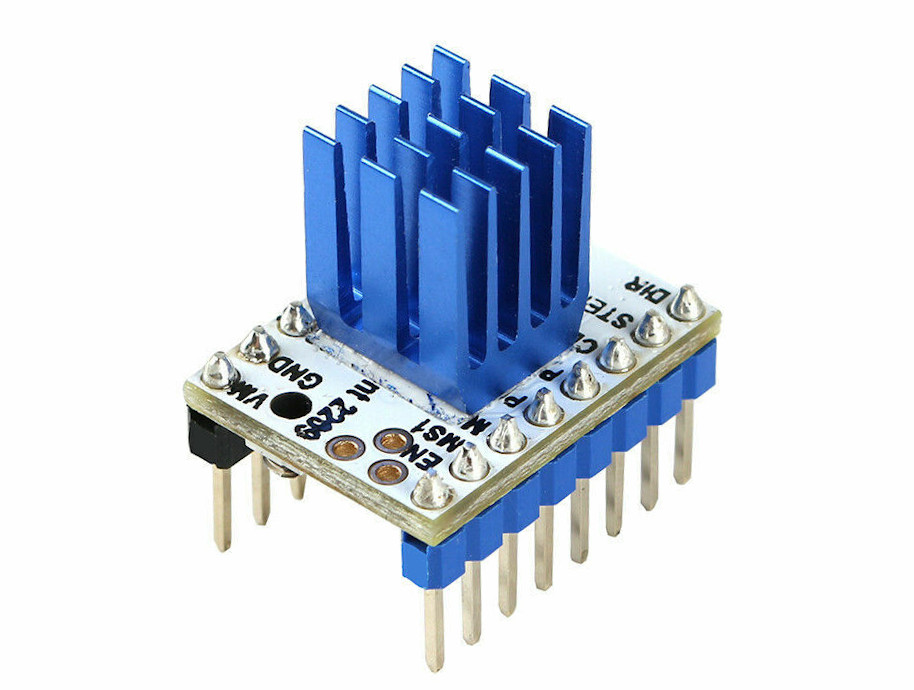
\includegraphics[width=6cm]{figs/TMC2209.jpg}
    \end{center}
    \caption{Controlador TMC2209}
    \label{fig:robSoldering}
\end{figure}\ 

\begin{table}[H]
\begin{center}
\begin{tabular}{|c|c|}
\hline
\textbf{Parámetros} & \textbf{Valores} \\
\hline
Nombre del controlador & TMC2209 \\
Voltaje lógico & 3 - 5V \\
Voltaje de alimentación & 5.5 - 28V \\
Microsteps & Hasta 1/256 \\
Corriente máx. de fase (RMS) & 2A \\
Pérdida de conducción (RDS) & 0.2$\Omega$ \\
Interfaz de comunicación & Pines CFG y UART \\
\hline
\end{tabular}
\caption{Especificaciones técnicas del TMC2209}
\label{cuadro:ejemplo}
\end{center}
\end{table}
    
\newpage
\section{Fuente de alimentación genérica}
\label{subsec:fuente_alimentacion}
Para alimentar el brazo se va a utilizar una fuente de alimentación genérica de 24 voltios y 6 amperios. Este tipo de fuentes pueden ser 
fácilmente adquiribles por internet por un precio aproximado de 15\euro. A pesar de esto, puede ser usada cualquier tipo de fuente capaz de 
entregar más de 20 vatios en el rango de voltaje 12-24v. Más adelante se aborda el uso de cargadores de ordenadores portátiles para alimentar el 
brazo.

\begin{figure} [h!]
  \centering    
  \subfigure[Fuente de alimentación 24v 5A]{\label{fig:pw24}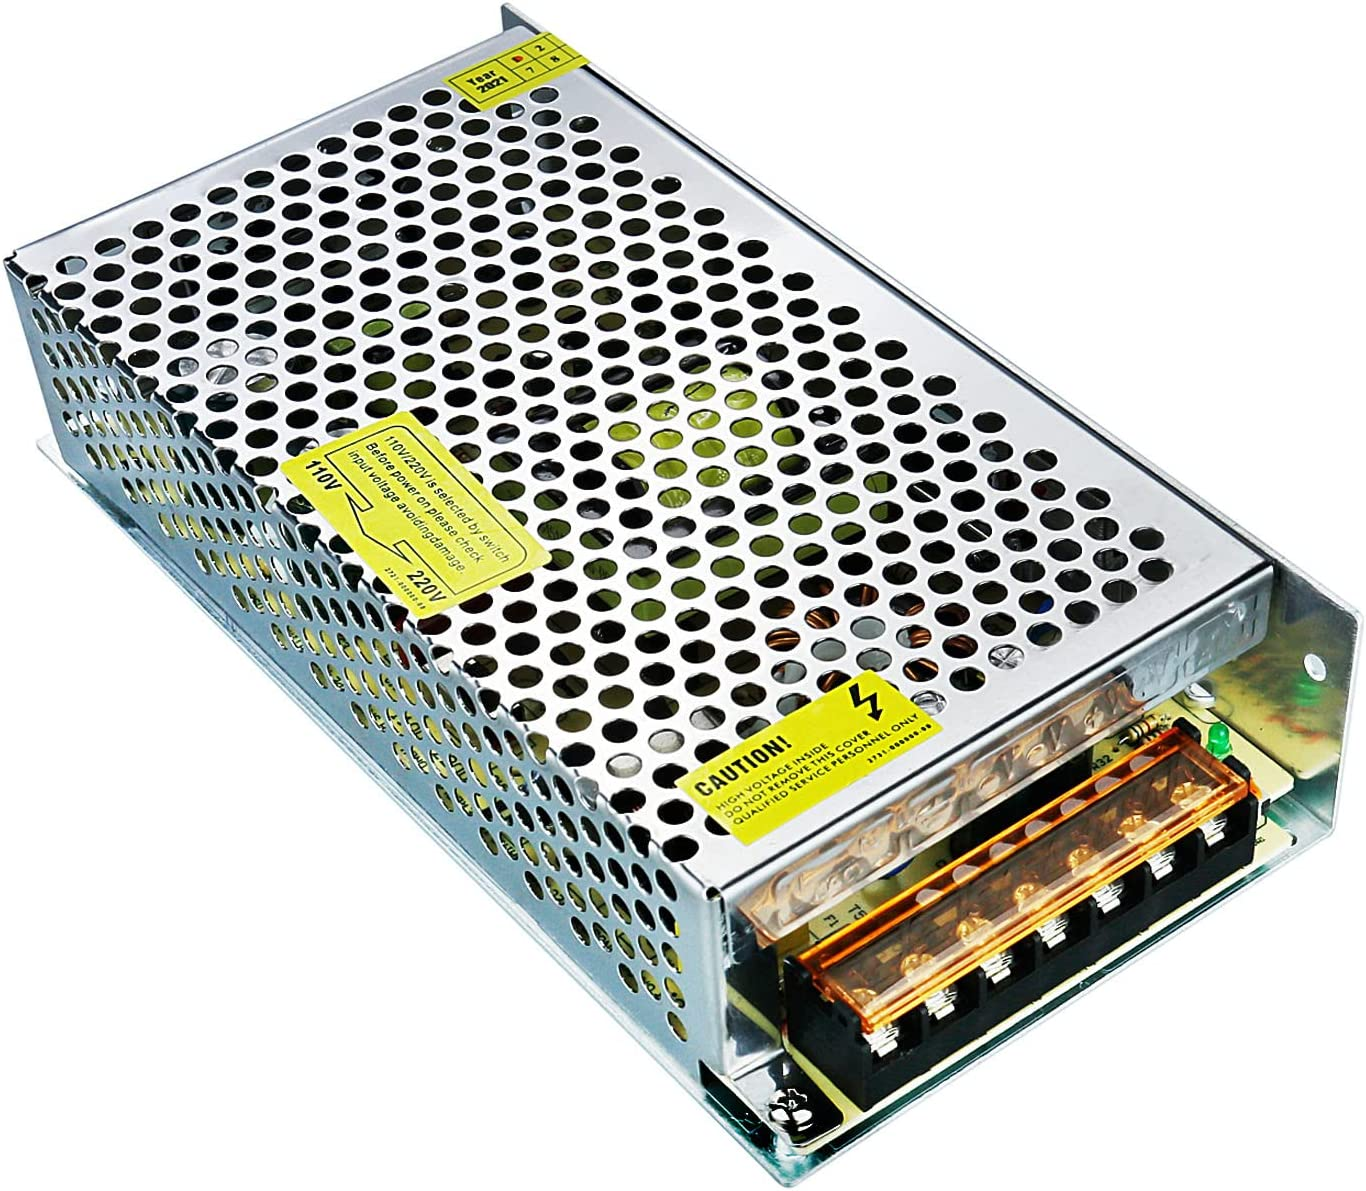
\includegraphics[width=0.55\linewidth ]{figs/pw24v.jpg}}
  \hspace{3cm}
  \subfigure[Cargador de portátil genérico]{\label{fig:pw19}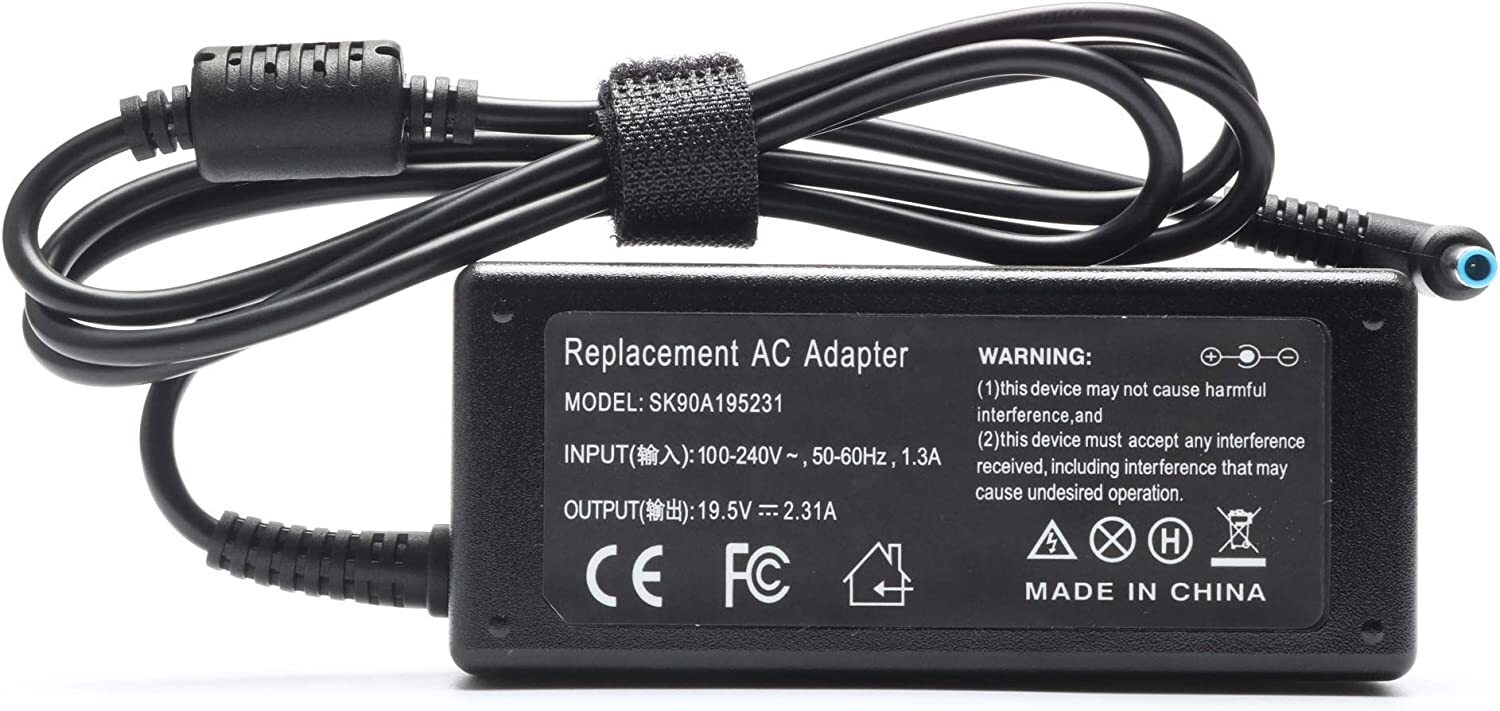
\includegraphics[width=0.55\linewidth]{figs/pw19v.jpg}}
  \caption{Métodos usados para alimentar el robot}
\end{figure}




\chapter{Desarrollo hardware del manipulador}
\label{cap:capitulo5}

\vspace{1cm}

En este capítulo se aborda el desarrollo necesario para, a partir de un concepto, acabar construyendo un prototipo real funcional. Se 
hace incisión en cada etapa necesaria para este cometido.


Escribe aquí un párrafo explicando brevemente lo que vas a contar en este capítulo. En este capítulo (y quizás alguno más) es donde, por fin, describes detalladamente qué has hecho y qué experimentos has llevado a cabo para validar tus desarrollos.

\section{Concepto}
En esta sección se expone como ha sido el proceso de encontrar y definir la idea fundamental del robot, en función de 
los objetivos propuestos, evaluando las distintas opciones para encontrar el que mejor se adapte. Se trata de balance

Primero, se debe conocer el numero de grados de libertad que se ajuste a los requisitos establecidos en la sección \ref{sec:requisitos}. En base 
a los requisitos 1 y 5, que limitan en cuanto a precio de fabricación y complejidad de los mismos, se ha decidido limitar los grados de 
libertad a un máximo de 4. 

hablamos del tipo de joints que existente

Con 4 grados de libertad vamos mal pero se puede.
Tipos:
Scara

RR

Basado en paralelos

\section{Modelo alámbrico}
\subsection{En qué consiste}
\label{subsec:eqc_mod_alambrico}
El modelo alámbrico es una forma de analizar el movimiento de un sistema mecánico compuesto por ejes y eslabones. Este 
enfoque simplifica la representación visual al destacar las relaciones espaciales entre las diferentes partes del sistema mediante 
líneas y conexiones simbólicas, en lugar de mostrar detalles realistas del manipulador. 
\begin{figure} [h!]
  \begin{center}
    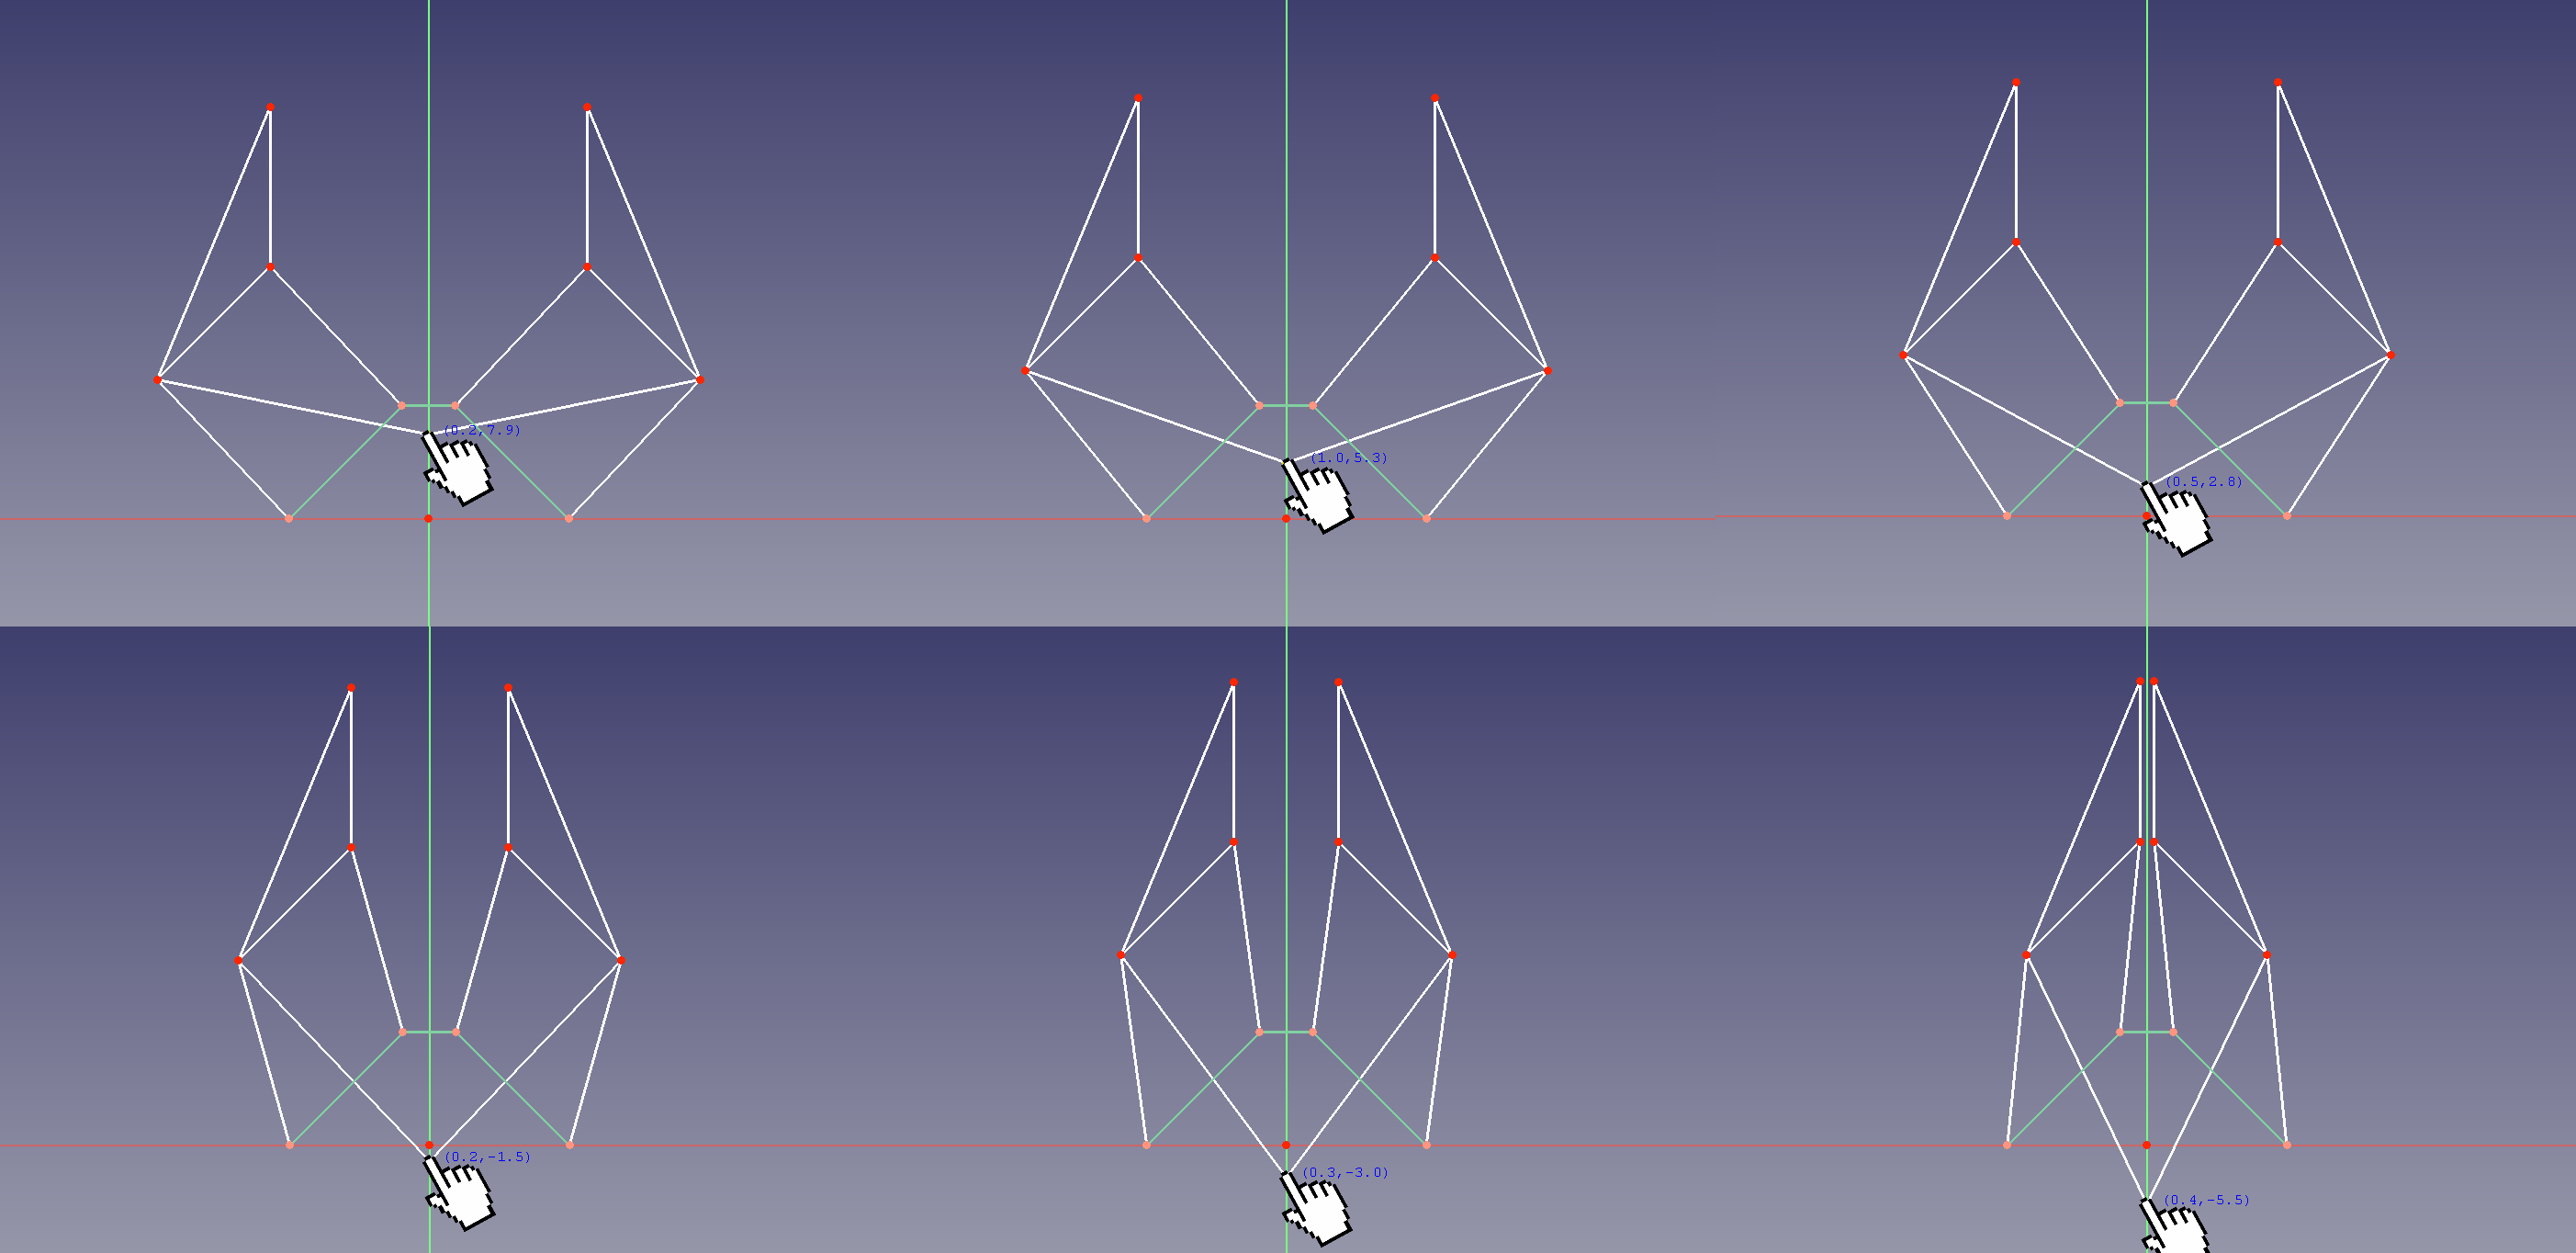
\includegraphics[width=15cm]{figs/pinza_evol.png}
  \end{center}
  \caption{Pinza paralela con 1 grado de libertad}
  \label{fig:mod_pinza_figure}
\end{figure}\ 

\subsection{Modelo alámbrico del brazo MeArm \ref{fig:mearm}}
\label{subsec:mod_mearm}


\section{Dinámica}

\section{DH}

\section{Bocetos}

\section{Diseño CAD}

\section{Diseño CAD}


\begin{code}[h]
\begin{lstlisting}[language=C++]
void Memory::hypothesizeParallelograms () {
  for(it1 = this->controller->segmentMemory.begin(); it1++) {
    squareFound = false; it2 = it1; it2++;
    while ((it2 != this->controller->segmentMemory.end()) && (!squareFound)) {
      if (geometry::haveACommonVertex((*it1),(*it2),&square)) {
        dist1 = geometry::distanceBetweenPoints3D ((*it1).start, (*it1).end);
        dist2 = geometry::distanceBetweenPoints3D ((*it2).start, (*it2).end);
      }
    // [...]
\end{lstlisting}
\caption[Función para buscar elementos 3D en la imagen]{Función para buscar elementos 3D en la imagen}
\label{cod:codejemplo}
\end{code}

En el Código \ref{cod:codejemplo2} vemos un ejemplo escrito en \texttt{Python}.

\begin{code}[h]
\begin{lstlisting}[language=Python]
def mostrarValores():
    print (w1.get(), w2.get())

master = Tk()
w1 = Scale(master, from_=0, to=42)
w1.pack()
w2 = Scale(master, from_=0, to=200, orient=HORIZONTAL)
w2.pack()
Button(master, text='Show', command=mostrarValores).pack()

mainloop()
\end{lstlisting}
\caption[Cómo usar un Slider]{Cómo usar un Slider}
\label{cod:codejemplo2}
\end{code}

\section{Verbatim}

Para mencionar identificadores usados en el código ---como nombres de funciones o variables--- en el texto, usa el entorno literal o verbatim \verb|hypothesizeParallelograms()|. También se puede usar este entorno para varias líneas, como se ve a continuación:

\begin{verbatim}
void Memory::hypothesizeParallelograms () {
  // add your code here
}
\end{verbatim}

\section{Ecuaciones}

Si necesitas insertar alguna ecuación, puedes hacerlo. Al igual que las figuras, no te olvides de referenciarlas. A continuación se exponen algunas ecuaciones de ejemplo: Ecuación \ref{ec:ec1} y Ecuación \ref{ec:ec2}.

\begin{myequation}[h]
\begin{equation}
H = 1 - \frac{\sum_{i=0}^{N}\frac{(\frac{d_{j_s} + d_{j_e}}{2})}{N}}{M}
\nonumber
\label{ec:ec1}
\end{equation}
\caption[Ejemplo de ecuación con fracciones]{Ejemplo de ecuación con fracciones}
\end{myequation} 

\begin{myequation}[h]
\begin{equation}
v(entrada)= \left\{
	\begin{array}{lcc}
		0 & \mbox{if} & \epsilon_t < 0.1\\
		K_p\cdot{(T_{t}-T)} & \mbox{if}& 0.1 \leq \epsilon_t < M_t\\
		K_p \cdot M_t & \mbox{if}& M_t < \epsilon_t
	\end{array}
\right.
\label{ec:ec2}
\end{equation}
\caption[Ejemplo de ecuación con array y letras y símbolos especiales]{Ejemplo de ecuación con array y letras y símbolos especiales}
\end{myequation}

\section{Tablas o cuadros}

Si necesitas insertar una tabla, hazlo dígnamente usando las propias tablas de \LaTeX, no usando pantallazos e insertándolas como figuras... En el Cuadro \ref{cuadro:ejemplo} vemos un ejemplo.

\begin{table}[H]
\begin{center}
\begin{tabular}{|c|c|}
\hline
\textbf{Parámetros} & \textbf{Valores} \\
\hline
Tipo de sensor & Sony IMX219PQ[7] CMOS 8-Mpx \\
Tamaño del sensor & 3.674 x 2.760 mm (1/4" format) \\
Número de pixels & 3280 x 2464 (active pixels) \\
Tamaño de pixel & 1.12 x 1.12 um \\
Lente & f=3.04 mm, f/2.0 \\
Ángulo de visión & 62.2 x 48.8 degrees \\
Lente SLR equivalente & 29 mm \\
\hline
\end{tabular}
\caption{Parámetros intrínsecos de la cámara}
\label{cuadro:ejemplo}
\end{center}
\end{table}



\clearpage
\thispagestyle{empty}

\printindex \nocite{*}
\appendix
\bibliographystyle{apalike} \bibliography{bibliografia}

\end{document}
